\documentclass[a4paper, 12pt]{report}
\usepackage[margin=2.5cm]{geometry}
\usepackage[utf8]{inputenc}
\usepackage[frenchb]{babel}
\usepackage[T1]{fontenc}
\usepackage{graphicx}
\usepackage{lettrine}
\usepackage{lmodern}
\usepackage{eso-pic}
\usepackage{tabularx}
\usepackage{titlesec}
\usepackage{colortbl}
\usepackage{xcolor}
\usepackage{setspace}
\usepackage{tikz}
\usepackage{hyperref}
\usepackage{stmaryrd}
\usepackage{subfig}
\usepackage{graphicx} 
\usepackage{caption}
\usepackage{mwe}
\usepackage{lipsum}
\usepackage{filecontents}
\usepackage{wrapfig}
\usepackage{url}
\hypersetup{
    colorlinks=true,
%     linkcolor=blue,
    citecolor=black,
    filecolor=black,
    linkcolor=black,
    urlcolor=black
}


\definecolor{olivegreen}{rgb}{0,0.5,0}

\titleformat{\chapter}[hang]{\bf\LARGE}{\thechapter}{0pc}{ - }
\titleformat{\section}[hang]{\bf\Large}{\thesection}{0pc}{ - }
\titleformat{name=\chapter,numberless}[hang]{\bf\LARGE}{}{0pc}{}
\titleformat{name=\section,numberless}[hang]{\bf\Large}{\thesection}{0pc}{}
%%%%%%%%%%%%%%%%%%%%%%%%%%%%%%%%%%%%%%%%%%%%%%%%%%%%%
%%%%%%%%%%%%% PROJECT TITLE%%%%%%%%%%%%%%%%%%%%%%%%%

\title{Rapport de Stage - 2018 }


%%%%%%%%%%%%%%%%%%%%%%%%%%%%%%%%%%%%%%%%%%%%%%%%%%%%




\begin{document}
%%%%%%%%%%%%%%%%%%
%%% First page %%%
%%%%%%%%%%%%%%%%%%

\begin{titlepage}
\begin{center}


\includegraphics[width=0.6\textwidth]{images/parisNanterre-logo}\\[1cm]

{\large Mémoire de stage de Master 1 MIAGE}\\[0.5cm]

{\large Stage réalisé à WATIZ}\\[0.5cm]

% Title
\rule{\linewidth}{0.5mm} \\[0.4cm]
{ \huge \bfseries Développement Front-End de site Web et d'interfaces pour des solutions de moteur de recherche visuelle \\[0.4cm] }
\rule{\linewidth}{0.5mm} \\[1.5cm]

% Author and supervisor
\noindent
\begin{minipage}{0.4\textwidth}
  \begin{flushleft} \large
    \emph{Étudiant :}\\
    Hani \textsc{Abdulwahab}
  \end{flushleft}
\end{minipage}%
\begin{minipage}{0.4\textwidth}
  \begin{flushright} \large
    \emph{Encadrants :} \\
    Mme.~Sonia \textsc{GUEHIS}\\
    M.~Marc \textsc{DÉCOMBAS}
    M.~Rémy \textsc{VILLECROZE}
    
  \end{flushright}
\end{minipage}

\vfill

% Bottom of the page
{\large Version 0.1 du\\ \today}

\end{center}
\end{titlepage}

\tableofcontents
\listoffigures
\chapter*{Remerciements}
Pour leur soutien, leur disponibilité et leur écoute tout au long de ce master MIAGE, je souhaite tout d'abord remercier Monsieur le professeur POIZAT, Monsieur le professeur GUYON et Madame CHAU, chargée d’insertion professionnelle. \\

Pour m’avoir accordé sa confiance pour la réalisation de ce projet intéressant, je tenais à remercier Madame GUEHIS, responsable de mon stage.\\

Pour m’avoir accompagné, conseillé et formé tout au long de ce stage, je tenais à remercier Monsieur VILLECROZE, encadrant mon stage.\\

Pour l’aide technique, et les réponses à mes interrogations, j’adresse aussi mes remerciements à Monsieur DÉCOMBAS, ainsi que Monsieur CAPRA.\\

Pour leur aide, les informations sur les stages et les offres, je tiens à remercier également toute l'équipe administrative du master MIAGE. \\

Mes plus profonds remerciements vont à mes parents. Tout au long de mon cursus, ils m’ont toujours soutenu, encouragé et aidé, malgré la distance qui nous éloigne à présent. Je remercie en particulier mon cousin le Docteur Alain ABDULWAHAB et sa famille, pour m’avoir soutenu dans mes efforts depuis mon arrivée en France.  \\

Je remercie tous mes plus proches amis, en ayant une pensée pour Nicolas ROUGE à qui je souhaite réussite et bonheur. \\

Plus personnellement, je remercie ma bien-aimée, Zuleyha KABA, pour son soutien infini, son écoute et surtout son amour qui m’a été essentiel durant ces années. 


\chapter{Introduction}
La recherche visuelle des produits est la pratique par laquelle, à partir du chargement d’une photo ou d’une capture d’écran d’un produit, un moteur de recherche ou une application mobile spécialisée met à disposition une liste de sites web marchands ou de pages proposant un produit similaire à la vente. La recherche visuelle est une pratique qui s'annonce comme une tendance lourde au même titre que la recherche vocale.
Elle deviendra un enjeu dans de nombreux secteurs, notamment dans celui de la mode. Ce secteur capitalise sur le grand nombre d’utilisateurs de mobiles et sur l’avènement des applications de partage de photos et de vidéos. Beaucoup de facteurs rendent la recherche visuelle efficace. Certains d’entre eux sont d’ordre physiologique. En effet, le cerveau traite 60 000 fois plus vite les images que les textes, 90\% de l'information envoyée au cerveau est visuelle et 93\% de la communication humaine est visuelle \cite{0}. Du fait de la grande utilisation de l’internet, les consommateurs sont devenus plus autonomes, plus axés sur la recherche et de plus en plus exigeant vis-à-vis de la technologie. Les consommateurs effectuent de plus en plus une recherche sur internet pour trouver une photo du produit avant d'acheter celui-ci.\\

L’entreprise française Watiz, crée en 2016, prépare aujourd’hui de nouvelles solutions permettant une généralisation de cet usage sur de nouveaux supports, les réseaux sociaux et les plateformes de streaming notamment. Elle s'est fait connaître avec succès pour ses produits innovants.\\

Dans le cadre de mon Master M1 MIAGE à l'Université Paris Nanterre, j'ai souhaité réaliser mon stage dans cette entreprise répondant aux enjeux des nouvelles technologies, avec la recherche visuelle. Les missions de développement d’un site web responsive et de développement d’un plug-in navigator m'ont attiré particulièrement car j’ai pu améliorer mes connaissances techniques en développement web front-end et mon esprit créatif avec le design (UX/UI user expérience et user interface expérience).\\

Nous verrons ainsi, au travers de ce rapport, la présentation de l'entreprise et de son secteur. Puis, nous aborderons les méthodes que j’ai pu utilisé pour réaliser et gérer nos projets ainsi que les concepts nécessaires à acquérir pour atteindre les objectifs de mes missions. 
Ensuite, nous décrirons les différents projets auxquels j’ai participé lors de ce stage avant de dresser un bilan professionnel et personnel dans le dernier chapitre. 
\chapter{Présentation de l'entreprise}
\section{Historique}
Créée en septembre 2016, Watiz est une start-up normande spécialisée dans le traitement de l'image et dans la reconnaissance visuelle. Elle développe une technologie de moteur de recherche nouvelle génération qui repose sur une technologie de détection et de ré-identification en temps réel d'objets dans des flux image et vidéo.

Watiz est hébergée par la pépinière Smart’up, une pépinière est portée par la CCI portes de Normandie, Evreux Portes de Normandie et la base aérienne 105. 
Depuis janvier 2018, Watiz est incubée à l’IMT Starter, un incubateur rattaché à TélécomSud Paris. Watiz y dispose d’un bureau secondaire où j’ai effectué mon stage.
\section{L’équipe}
Les trois fondateurs Julien CAPRA (HEC Entrepreneurs, PhD Paris XI, Ingénieur ECPM), Rémy VILLECROZE (PhD Lyon Claude Bernard 1, Ingénieur Telecom Sud- Paris) et Marc DECOMBAS (PhD Telecom Paris, Ingénieur Telecom Sud Paris) comptent sur leurs liens privilégiés avec le monde de la recherche académique pour mettre en place des solutions toujours plus innovantes dans les technologies du traitement de l’image. 
En plus des trois fondateurs, l’équipe est composée également
d’une ingénieure R\&D diplômée de l’ENSIEE qui aide à développer et à produire les algorithmes, et de 
deux stagiaires ingénieurs spécialisés en développement et en intelligence artificielle.

Watiz est portée par une équipe complémentaire et expérimentée disposant à la fois de solides expériences dans les domaines académique et industriel.
  
En tant que stagiaire web front-end, j’ai intégré l’équipe technique sous la direction de Marc DÉCOMBAS et je travaillais en étroite collaboration avec  Rémy VILLECROZE, le responsable produit. 
\section{L’entreprise aujourd’hui}
Watiz est un fournisseur de technologie pour les grands comptes et pour les industriels.
La société est en train de lancer son premier produit : un SDK de moteur de recherche visuelle dédié à la mode.
En attendant la commercialisation de ce premier produit, l’entreprise valorise son expertise dans le domaine de la vision par ordinateur et en intelligence artificielle via des missions de conseils ou de prototypage auprès d’industriels et de PME françaises. Les missions sont variées et touchent différents secteurs : analyse satellitaire, robot testeur d’UX, sécurité télésurveillance, etc.

\section{La vision des fondateurs}
Watiz a pour but de simplifier l’accès à l’information en proposant une alternative simple et complémentaire aux moteurs de recherche classiques permettant de retrouver un objet sans initier de recherche textuelle.
Aujourd’hui, Watiz a choisi de lancer un premier SDK de moteur de recherche visuelle intégré dans des applications mobiles de marques ou de distributeurs multimarques.
Les fondateurs sont convaincus que la recherche visuelle est une pratique qui deviendra une tendance lourde à l’avenir dans le domaine de la mode. Ils préparent aujourd’hui de nouvelles solutions permettant une généralisation de cet usage sur de nouveaux supports, les réseaux sociaux et les plateformes de streaming notamment.
\section{Les solutions de Watiz}
\subsection{Watstyle}
En plaçant le monde comme source d'inspiration, WatStyle permet de proposer aux utilisateurs d’accéder instantanément à une sélection de produits à partir d’une simple photo. Plus besoin de connaître le nom d’un article, le consommateur le retrouve uniquement grâce à son apparence.\\
Watstyle est un SDK qui:
\begin{itemize}
\item S'intègre dans les applications clients.
\item Permet de prendre ou de charger une photo dans l’application.
\item Analyse et reconnaît les vêtements présents sur la photo.
\item Redirige l’utilisateur  vers les bonnes références du catalogue Client.
\end{itemize}
\subsection{Epick}
Epick est un plug-in navigateur qui permet de retrouver en temps réel des vêtements apparaissant dans un flux vidéo. En mettant sur pause sa vidéo, l’utilisateur découvre les articles détectés par Epick et en cliquant dessus, il peut le ranger dans un panier virtuel. En sélectionnant ensuite dans son panier, l’utilisateur est redirigé vers le site de e-commerce correspondant.
\section{La technologie}\label{sec:technologie}
Watiz a pour ambition de développer une nouvelle technologie de moteur de recherche visuelle permettant de retrouver facilement n’importe quel vêtement aperçu dans un flux d’images, animé ou non.

Afin de réaliser ce moteur de recherche objet, Watiz s’est appuyée sur les connaissances de ses fondateurs en traitement de l’image et en intelligence artificielle pour déployer ses briques technologiques. Pour la plupart de ces briques, Watiz a utilisé des algorithmes basés sur de l’apprentissage par réseaux de neurones (machine et deep learning), une technologie inspirée du fonctionnement du cerveau qui permet à la machine d'apprendre des notions et des comportements (ici la reconnaissance d'objets) à partir d'un très grand nombre d’exemples et de situations.

De nombreux domaines de la reconnaissance visuelle ont connu un réel essor ces dernières années pour arriver à des performances similaires à celles d’un être humain (par exemple la reconnaissance de caractères et de chiffres et la détection de visages sont des sujets maîtrisés).

La reconnaissance d’objets est, quant à elle, beaucoup moins mature. À cette date, il n’existe pas de technologie capable d’attaquer le problème de la reconnaissance d’objets, même dans des poses contraintes, c’est-à-dire avec des angles de vues maîtrisés, qui donne des performances comparables aux performances humaines.

L’un des principaux obstacles aujourd’hui tient à la quantité de données qu’il faut prendre en compte dans ce problème : une grande diversité dans les objets et des objets similaires entre eux.

Pour faire face à cette problématique, Watiz a choisi de construire sa technologie en s’appuyant sur des algorithmes permettant :
 \begin{itemize}
\item De détecter et classifier (c’est-à-dire être en mesure de ranger l’objet détecté dans une catégorie) un à plusieurs objets en temps réels dans un flux vidéo.
\item De suivre ces objets dans le temps malgré des phénomènes d’occlusion ou de déformation (objet qui disparaît ou se déforme dans le temps).
\item De comparer ces objets détectés à des bases de données décrites par des descripteurs de nouvelle génération. Un descripteur est un vecteur qui permet de caractériser un objet à partir de données haut niveau (la couleur, la forme) ou bas niveau (description très locale ; ce type de descripteurs est bien détaillé dans la littérature). Avec l'avènement du deep learning et des réseaux convolutifs, la société Watiz a préféré construire ses propres descripteurs ayant la particularité d’associer descripteurs bas et haut niveau en fonction de l’avancement dans les couches de convolution.
\item De traiter à grande échelle les données fournies par l’analyse vidéo (projet CBORBIG en partenariat avec la SATT Paris-Saclay).
\end{itemize}
Aujourd’hui, plusieurs de ces algorithmes sont déjà opérationnels et ont éprouvés dans des cas d’usages industriels lors de missions de prestations.
\section{Problématique du stage}
L'objectif du stage était de finaliser le développement d’APIs et de SDK qui permettent de retrouver des objets en temps réel dans des images et des vidéos. 
Mes principales missions ont concerné la refonte de l’esthétique générale des produits Watiz, ciblant principalement le site vitrine de Watiz et l’extension Chrome Epick.

J’étais en charge de la maquette des sites Web et de l’uniformisation des différentes IHM. Attentif à la question du responsive design, j’ai amélioré et vérifié le bon fonctionnement des interactions proposées sur différents appareils (ordinateur, tablette, téléphone portable...) et différents navigateurs. 

Les missions réalisées jusqu'à présent sont : 
\begin{itemize}
\item \textbf{Le développement d’un site web:}
La société avait besoin d’un nouveau site qui devait être mis en ligne avant Vivatechnology, un événement international auquel participait Watiz en tant qu’exposant.
L’ancien site était obsolète et ne présentait pas le nouveau produit, WatStyle. La mission consistait à analyser les besoins en communication de la société et à comprendre ce qu’elle reprochait à son ancien site. Il fallait ensuite concevoir et développer un site internet répondant à ces critères et former les responsables pour les futures mises à jour du site.

\item \textbf{La finalisation d’un plug-in Google Chrome Epick:} 
Ma mission a consisté initialement à développer les pages de Landing et de Welcome concernant le téléchargement de l'extension de Google Chrome. J’ai ensuite participé à développer certaines fonctionnalités de l’extension Epick. Le projet Epick est toujours en cours. Les missions actuelles sont l'optimisation et la généralisation à d'autres sites du POC Epick. 


\end{itemize} 

\chapter{Méthodes et outils de travail}
\section{Les aspects techniques}
\subsection{Environnement de développement}
\begin{itemize}
\item \textbf{Webstorm \& Brackets:}
Pour le développement web front-end, j'ai utilisé Webstorm qui  est un IDE pour les langages Web (HTML, CSS et JavaScript), développé par l'entreprise JetBrains. 
Ensuite, j’ai utilisé Brackets qui est un éditeur open source pour le web design et le développement sur des technologies Web et qui fournit un future, Quick edit, une fonctionnalité offrant aux développeurs de modifier, directement en ligne, du code CSS, JavaScript :
\begin{itemize}
\item Mise à jour du code HTML et CSS, dans le navigateur web, en temps réel sans rechargement ;
\item  Surbrillance des éléments : le ou les éléments sélectionnés sur Brackets sont affichés en surbrillance dans le navigateur web.
\end{itemize} 

\item \textbf{Photoshop} 
est un outil de création graphique puissant. Très flexible, avec ses nombreux outils adaptés, il nous permet de créer ensemble tous les éléments d’un site responsive.
J'utilise des maquettes graphiques pour me donner une idée très précise de l'aspect qu'aura mon site à la fin du projet, avant de commencer le code.
C'est la réalisation de ces maquettes que nous allons maintenant aborder ensemble dans le paragraphe ~\ref{subsec:MA}.
\end{itemize} 
\subsection{Le serveur OVH}
OVH est une entreprise française spécialisée dans les services de cloud computing.
La société Watiz utilise OVH pour héberger son site web , ainsi que le service cloud pour l’algorithme de  moteur de recherche.
Pour déployer le code en prenant en compte les modifications, il faut se connecter au serveur OVH de Watiz. Pour cela, ayant besoin d’un environnement Linux,  j’ai configuré une clef SSH à partir d’une machine virtuelle (VmWare).
Une fois connecté au serveur, je pouvais git puller (c’est-à-dire rapatrier les modifications du git sur le serveur OVH) dans le terminal distant.
\subsection{Les langages utilisés}
\begin{itemize}
\item \textbf{HTML} signifie « HyperText Markup Language » que l'on peut traduire par « langage de balises pour l’hypertexte ». Il est utilisé afin de créer et de représenter le contenu d’une page web. 
\item \textbf{CSS} Cascading Style Sheets est un langage de feuille de style utilisé pour décrire la présentation d’un document écrit en HTML ou en XML. CSS décrit la façon dont les éléments doivent être affichés, à l’écran, sur du papier ou sur un autre support. 
\item \textbf{Javascript} est un langage de script léger, orienté objet et interprété, principalement connu comme le langage de script des pages web, mais il est aussi utilisé dans de nombreux environnements extérieurs aux navigateurs web, tel que Node.js. JavaScript est principalement utile lorsqu’il s’agit d’améliorer et d’étendre le comportement des pages. Ce langage vient compléter le HTML et le CSS, en y ajoutant une couche d’interactivité. 
\item \textbf{JQuery} est une bibliothèque JavaScript créée pour faciliter l’écriture de scripts côté client et permet de profiter d’une plus grande compatibilité avec les différents navigateurs. Il est à l’heure actuelle le framework front-end le plus utilisé au monde.
\item \textbf{Framework (Bootstrap)} Le mot Framework est un mot anglais signifiant « cadre de travail ». Il s’agit en quelque sorte d’une boîte à outils qui a été conçue par d’autres programmeurs qui ont déjà travaillé sur des projets similaires, en vue de faciliter la tâche aux autres programmeurs afin qu’ils puissent se concentrer sur l’essentiel, leur logique métier. Un framework web est donc un ensemble d’outils qui forme un tout cohérent que l’on a juste à assembler selon nos besoins pour faire un site robuste, maintenable et durable. L’intégrateur pourra, par exemple, décider de démarrer un projet avec un framework front-end comme Bootstrap ou Foundation. 
\end{itemize} 
\section{Gestion de projet}
\subsection{Les méthodes agiles }
\begin{figure}[!ht]
\begin{center}
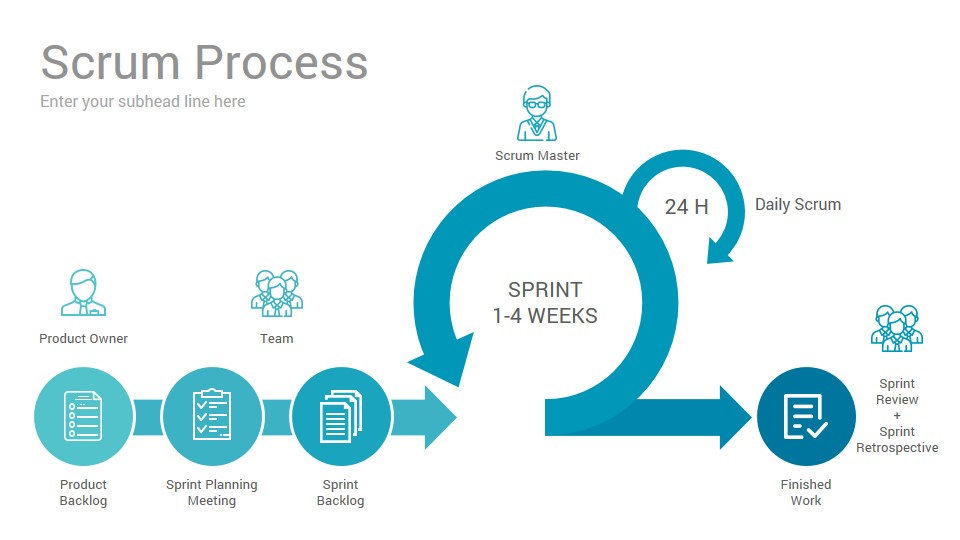
\includegraphics[height=7cm]{images/Scrum-Process.jpg}
\caption{Scrum Framwork}
\label{fig:3.1}
\end{center}
\end{figure}
Les méthodes agiles décrivent un ensemble de pratiques dans la gestion d’un projet. Elles impliquent au maximum le client et permettent une grande réactivité à ses demandes. Elles reposent sur un cycle de développement itératif, incrémental et adaptatif et doivent respecter une base de pratiques communes ou complémentaires.
La société Watiz travaille  en agilité en appliquant la méthode Scrum [ figure~\ref{fig:3.1} ].
La durée d’un sprint est fixée à 2 semaines dans le cadre de projet. L’objectif générique associé à chaque sprint consiste à transformer les exigences constituant le périmètre de ce dernier en fonctionnalités utilisables.
Avant de démarrer un sprint, nous sélectionnons les éléments de la liste ordonnancée des exigences (Product Backlog) qu’elle pense pouvoir réaliser dans le délai associé au sprint. Au cours de ce dernier, le Product Owner et l’équipe de développement collaborent étroitement pour atteindre les objectifs fixés. 
A la fin du Sprint, nous présentons les résultats de nos travaux sous la forme d’une démonstration des nouvelles fonctionnalités réalisées. Les feedbacks sont recueillis.
Chaque jour, nous faisons un « stand-up meeting » d'une durée maximum de 15 minutes en utilisant appear.in, l'équipe étant répartie sur deux sites.
Cette réunion, se faisant debout, permettant ainsi d'éviter de s’éterniser et d'aller directement à l'essentiel, est très importante. Elle nous permet quotidiennement de se synchroniser, de remonter les obstacles rencontrés, de s’entraider, de vérifier l’avancement du sprint. Elle contribue également à faire naître l’esprit d’équipe.
\subsection{Outils de gestion de projet}
Le terme logiciel de gestion de projet peut désigner différents types de logiciel ayant pour objectif de faciliter le travail de gestion de projet. Le travail des logiciels de gestion de projet est généralement d'automatiser des tâches de sauvegarde et/ou de la gestion du temps.
Il y a plusieurs méthodes utilisées pour la  gestion de projets. Au sein de la société Watiz, nous avons utilisé :

\begin{itemize}
\item \textbf{GitLab}
qui permet d’héberger et de gérer des projets web de A à Z. Présentée comme la plateforme des développeurs modernes, elle offre la possibilité de gérer nos dépôts Git et ainsi de mieux appréhender la gestion des versions de nos codes sources.
Github est payant pour les projets qui ne sont pas open source, et l'on ne peut bien évidemment pas modifier le code.

\item \textbf{Git}
où l'on « committe » (c'est-à-dire où l'on supervise) tous les nouveaux fichiers que l’on ajoute ou supprime, ainsi que les lignes modifiées dans le code. 
Les logiciels de gestion de version, comme Git, permettent de sauvegarder ses travaux sur le serveur, mais aussi de garder les informations liées à chaque modification du code et de pouvoir ainsi travailler à plusieurs sur le même projet.

\item \textbf{Trello}
qui est un outil de gestion de tâches. Afin d’être toujours à jour sur les projets potentiels, validés, rejetés, programmés, terminés, nous avons dédié un tableau de bord permettant de suivre l’état des projets en cours. Nous participons tous ensemble à l'attribution des tâches et au suivi de leur réalisations.
\item \textbf{Slack} qui est une plate-forme de communication collaborative propriétaire ainsi qu'un logiciel de gestion de projets. Nous utilisons Slack quotidiennement pour gérer nos projets et communiquer entre nous. 
Cette plateforme permet également de conserver une trace de tous les échanges et partager de fichiers au sein des conversations. Elle intègre  aussi des services externes comme Gitlab, Dropbox, Google Drive ou Trello pour centraliser le suivi et la gestion d'un projet.
\item \textbf{Appear.in} est un outil de collaboration vidéo qui permet de générer des salles de vidéoconférences à la demande sans inscription préalable.
\end{itemize} 
\section{Critères importants}
\subsection{UX/UI }
Le terme \textbf{UI} est l’abréviation d’user interface qui désigne l’interface utilisateur. Le rôle de l’UI designer consiste à concevoir une interface agréable par le biais duquel l’homme entre en contact avec le produit. Ce professionnel du design prend part aux discussions initiales avec l’UX designer et le client afin de déterminer les attentes de ce dernier, ses objectifs de communication et les besoins de l’utilisateur ciblé.\\
Le terme \textbf{UX} vient d’user expérience ou expérience utilisateur. Le travail de l’UX designer consiste donc à concevoir une interface accessible et facile à prendre en main pour tout type de support. D’ailleurs, ce professionnel est parfois désigné sous l’appellation ergonome en raison de la nature de sa mission. Pour ce faire, il analyse les souhaits du client et les besoins des cibles afin de concilier les deux. À partir des résultats, il conçoit l’architecture du site et les différentes fonctionnalités disponibles \cite{1}.
\subsection{La sémantique des balises }
La sémantique des balises permet de donner du sens et une structure à la page en utilisant les éléments (balises) appropriés. La sémantique décrit la valeur du contenu de la page, sans tenir compte de l’apparence ou de la mise en forme des informations. Le HTML sémantique est traité par les navigateurs courants et il est également beaucoup plus simple de travailler et de maintenir un code HTML sémantiquement correct puisque le document est découpé en parties claires et logiques. 
\subsection{La séparation entre la structure et la présentation}
 
L’un des objectifs majeurs des CSS est de permettre la mise en forme hors du document. Cette séparation fournit un certain nombre de bénéfices permettant d’améliorer l’accessibilité, de changer plus facilement de présentation et de réduire la complexité de l’architecture d’un document. 

\subsection{Un code organisé et réutilisable}

L’intégrateur doit produire un code propre, organisé et réutilisable, ceci afin de pouvoir être modifié facilement par un autre intervenant. Cette démarche commence dès la conception en cherchant à répondre aux besoins de l’utilisateur et uniquement aux besoins de l’utilisateur. Plusieurs techniques peuvent aider l’intégrateur à agir ainsi.

\subsection{Compatibilité cross-browser}
La compatibilité Cross-browser est la possibilité pour toute application web de supporter plusieurs navigateurs web. C’est-à-dire qu’un site doit être identique visuellement et proposer une expérience utilisateur égale sur tous les navigateurs. Il est donc nécessaire de tester et créer des correctifs spécifiques si besoin. Nous pouvons également faire le choix de ne plus prendre en compte certains navigateurs trop anciens ou obsolètes.

\subsection{Responsive design}

Un site web adaptatif, ou responsive, est un site web dont la conception vise à offrir une consultation confortable même pour des supports différents en s’adaptant au terminal du client \cite{2}. L’utilisateur peut ainsi, avec le même confort visuel, consulter le site à travers une large gamme d’appareils. Aujourd’hui, il en existe trois principaux : l’ordinateur de bureau classique, la tablette mobile et le smartphone. On peut, dans le cadre de la gestion de projet, décider de créer une version unique du site, et donc responsive, où choisir de créer une version supplémentaire spécialement adaptée à un format particulier.
\subsection{Accessibilité}
L’accessibilité, c’est permettre au plus grand nombre de profiter pleinement de votre site, quel que soit le matériel, les logiciels, les équipements particuliers ou le handicap de l’utilisateur. Il existe plusieurs normes à respecter, mais d’une façon générale, le plus simple et le plus efficace est de séparer le contenu du design dans des fichiers séparés. Les principales difficultés d’accessibilité sont : 
\begin{itemize}
\item La liaison bas débit qui ralentit le chargement de la page.
\item Le texte mal orthographié, utilisant des termes complexes ou pas adaptés au public visé.
\item Les navigateurs trop anciens ou peu connus. 
\item Un Site mal pensé, peu ergonomique où la navigation n’est ni intuitive ni cohérente ou basée uniquement sur des scripts.
\item Un Site ne prenant pas en compte les utilisateurs ayant un handicap visuel ou sonore. 
\end{itemize} 
\subsection{Référencement}
Le référencement est un ensemble de techniques consistant à améliorer le positionnement et la visibilité de sites dans les pages de résultats de moteurs de recherche ou d’annuaires et ainsi augmenter le trafic du site. Il s’articule autour de deux stratégies distinctes et complémentaires : le référencement naturel et le référencement payant. L’intégrateur web peut agir sur le référencement naturel en produisant un code qui décrit au mieux le contenu de la page et permet ainsi aux moteurs de recherches d’en parcourir l’intégralité avec facilité. On appelle cela de l’optimisation SEO. 
\pagebreak
\chapter{Les projets}
\section{Le projet Epick}
\subsection{Objectif et vision générale}
En tant que visionneurs de vidéos/films/ séries, nous nous sommes tous demandés un jour comment retrouver et acheter les mêmes vêtements que les personnages de séries. 
Cette démarche est généralement fastidieuse avec des mots clés présumés aléatoires sur Google “veste Ryan Gosling drive” avec au final très peu de résultats pertinents. 
Watiz a voulu simplifier ce processus en permettant à tout le monde d’acheter directement les vêtements qu'il voit dans une série ou dans un film. En un clic, vous pourrez avoir accès au costume de James Bond ou au t-shirt de Sheldon dans \textit{The Big Bang Theory}. 
En regardant une série, l’utilisateur pourra cliquer sur les vêtements qu’il aime et les ajouter à une liste de favoris, une wishlist, avant d'être redirigé sur le site de E-commerce pour pouvoir l’acheter. 

\subsection{Cas particulier et démonstrateur}\label{CP}
Pour démontrer l'intérêt et le potentiel marché d'Epick, nous avons voulu créer une preuve de concept, un POC, qui nous permettrait de travailler sur la faisabilité du projet, sur l'ergonomie et le design. 
Fort de cela, Watiz a créé un partenariat avec l’agence de communication Ogilvy. 
Le but n'était plus d’avoir cette fonctionnalité sur l'intégralité des sites Web mais seulement sur la plate-forme Netflix pour un seul épisode d'une série particulière. 
Une fois les contours du projet définis, les rôles ont été distribués, l’agence de communication allait s’occuper de l’aspect UI et UX alors que Watiz allait s’occupait de tout l’aspect développement. 
Au niveau de l’UX , plusieurs séances ont été organisées pour penser le produit.\\
\label{AN} La solution finale est partie de la volonté de ne pas interférer avec le design épuré de Netflix. Il a donc été validé que la proposition des produits interviendrait seulement lorsque l’utilisateur appuiera sur pause[ figure~\ref{fig:A} ]. En pause, des box proposeraient les vêtements disponibles sur cette image[ figure~\ref{fig:B} ]. En cliquant sur l'une d'elles, une animation apparaît pour faire attendre l’utilisateur [ figure~\ref{fig:C} ] puis, un cadre apparaît autour de l'image [ figure~\ref{fig:D} ]. Le résultat s’affiche dans une wishlist positionnée en bandeau vertical à droite de la vidéo [ figure~\ref{fig:E} ]. Ce résultat est une image du produit encadré. Ainsi l’utilisateur aura retrouver son produit sans être gêné dans le visionnage de sa vidéo[ figure~\ref{fig:F} ]. \\
En cliquant sur la wishlist[ figure~\ref{fig:H} ], un descriptif plus détaillé apparaît avec le titre du produit et son prix. On pourra ensuite accéder au E-shop en cliquant sur un bouton BUY ou sur l’image illustratrice. Il est possible également de retrouver des produits similaires en cliquant sur un bouton SIMILAR[ figure~\ref{fig:I} ].

%galerie d'image
\begin{figure}[htp]
  \centering
  \subfloat[vidéo en pause]{\label{fig:A}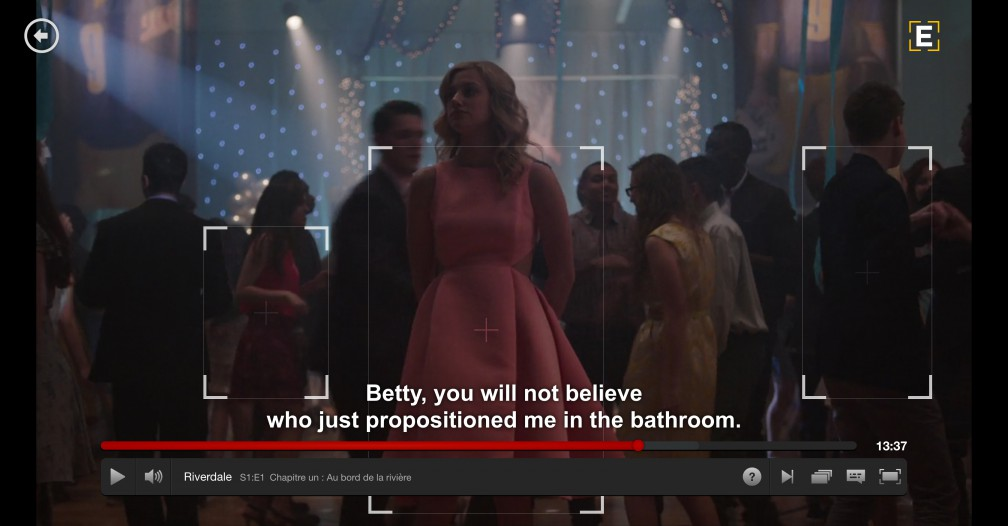
\includegraphics[height=3.8cm]{images/Step_01.jpg}}
  ~ %espace entre deux images sur une même ligne
  \subfloat[Cliquant sur une des BOX]{\label{fig:B}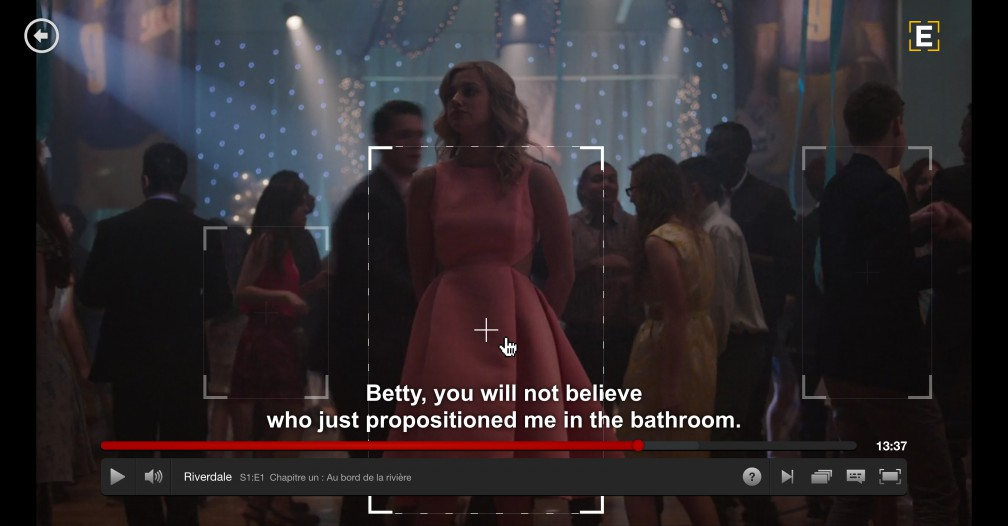
\includegraphics[height=3.8cm]{images/Step_02.jpg}}
  ~\\ %saute une ligne dans la galerie d'image
  
  \subfloat[Animation de chargement]{\label{fig:C}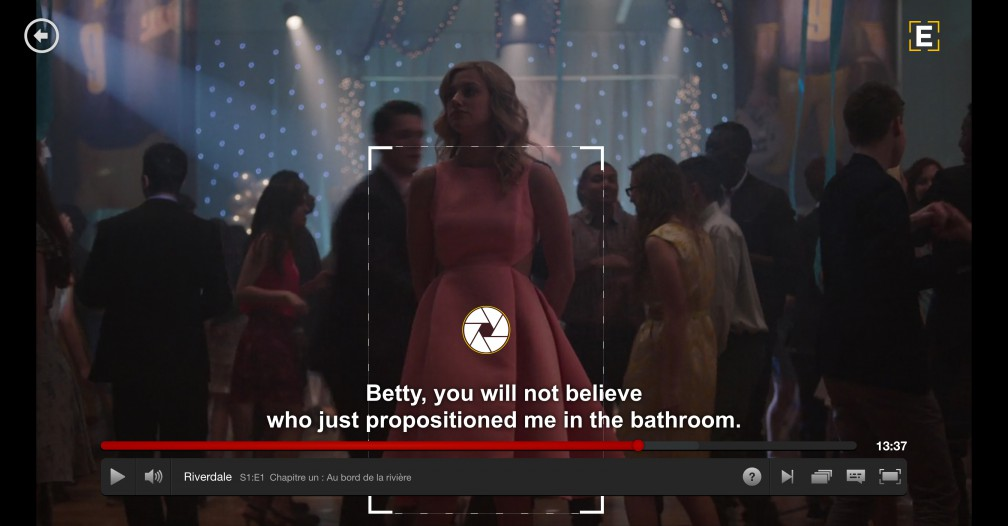
\includegraphics[height=3.8cm]{images/Steps_03.jpg}}
  ~
  \subfloat[Création d'un effet "Polaroïd"]{\label{fig:D}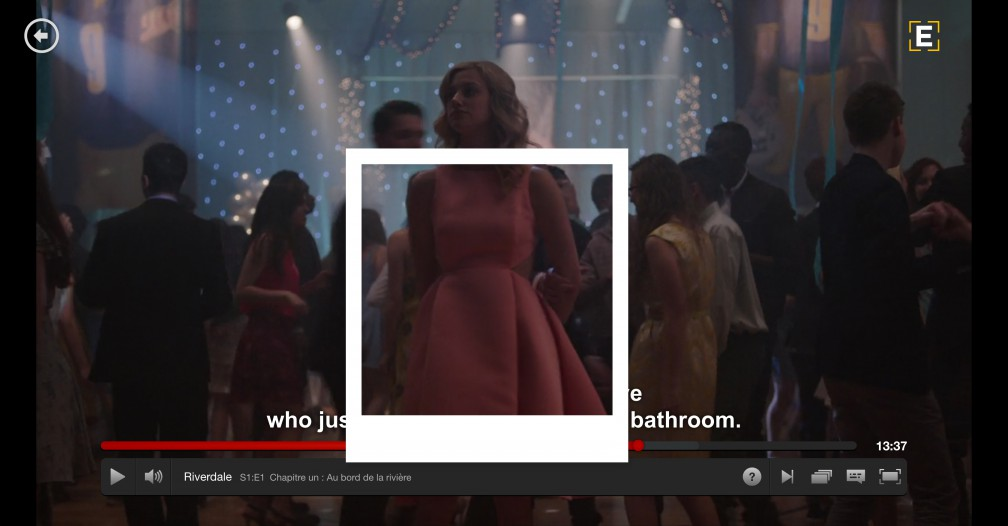
\includegraphics[height=3.8cm]{images/Steps_04.jpg}}
   ~\\ %saute une ligne dans la galerie d'image
  \subfloat[Enregistrement dans la wishlist]{\label{fig:E}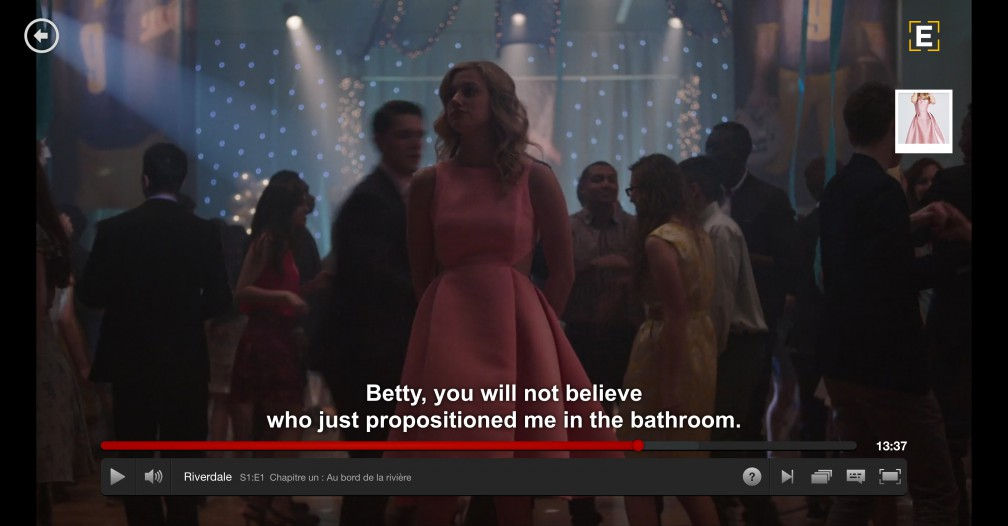
\includegraphics[height=3.8cm]{images/Steps_05.jpg}}
   ~
  \subfloat[Fermeture de la wishlist]{\label{fig:F}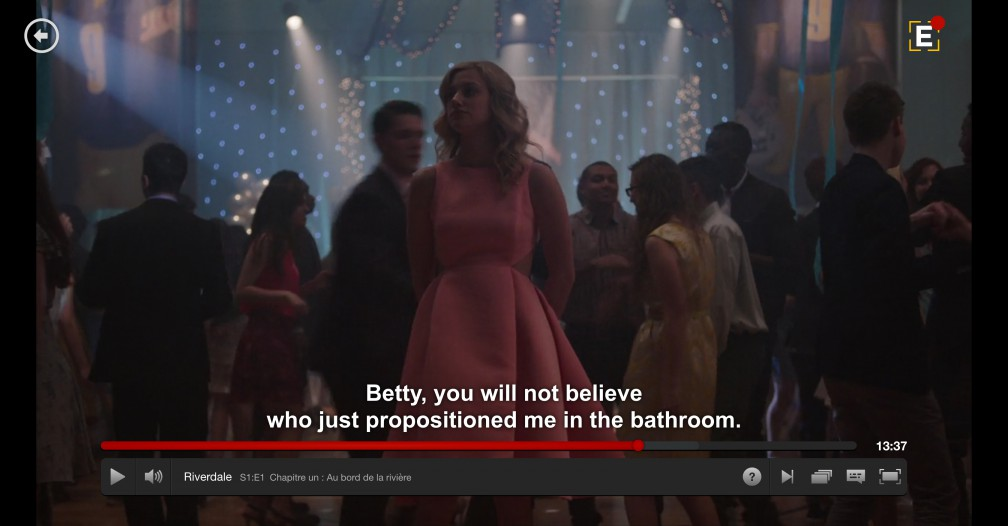
\includegraphics[height=3.8cm]{images/Steps_06.jpg}}
  ~\\ %saute une ligne dans la galerie d'image
  \subfloat[Interaction dans la wishlist]{\label{fig:G}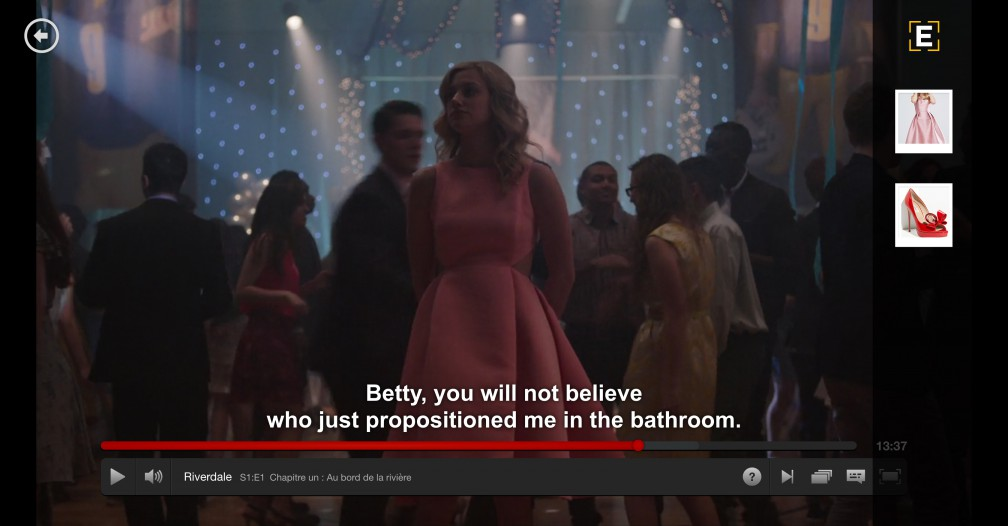
\includegraphics[height=3.8cm]{images/Steps_07.jpg}}
   ~
  \subfloat[Descriptif détaillé]{\label{fig:H}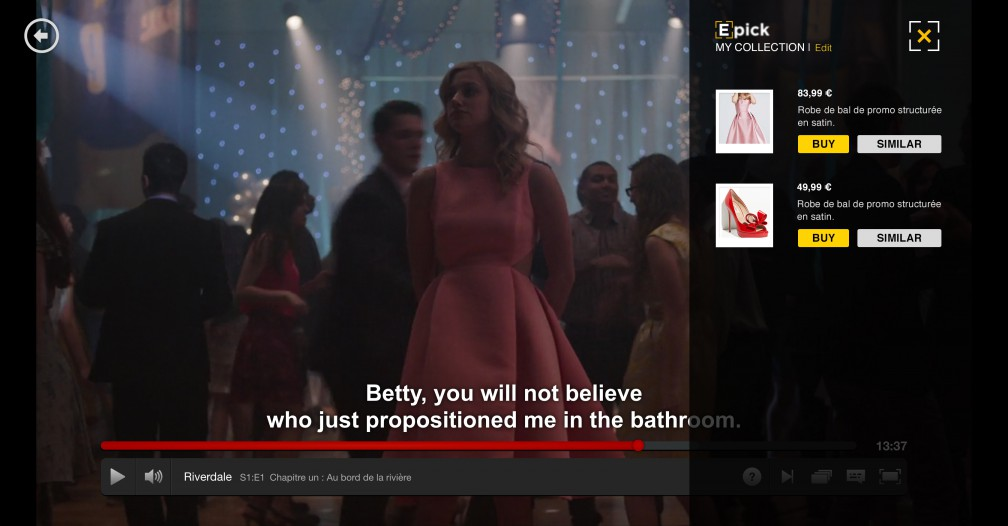
\includegraphics[height=3.8cm]{images/Steps_08.jpg}}
  ~\\ %saute une ligne dans la galerie d'image
  \subfloat[Présentation de produits similaires]{\label{fig:I}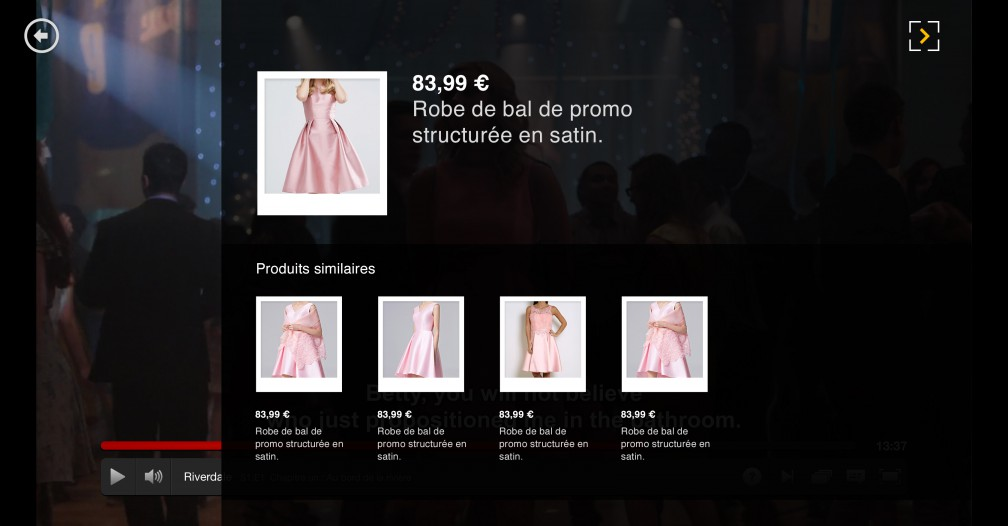
\includegraphics[height=3.8cm]{images/Steps_09.jpg}}
   ~
  \subfloat[Redirection vers e-shop]{\label{fig:J}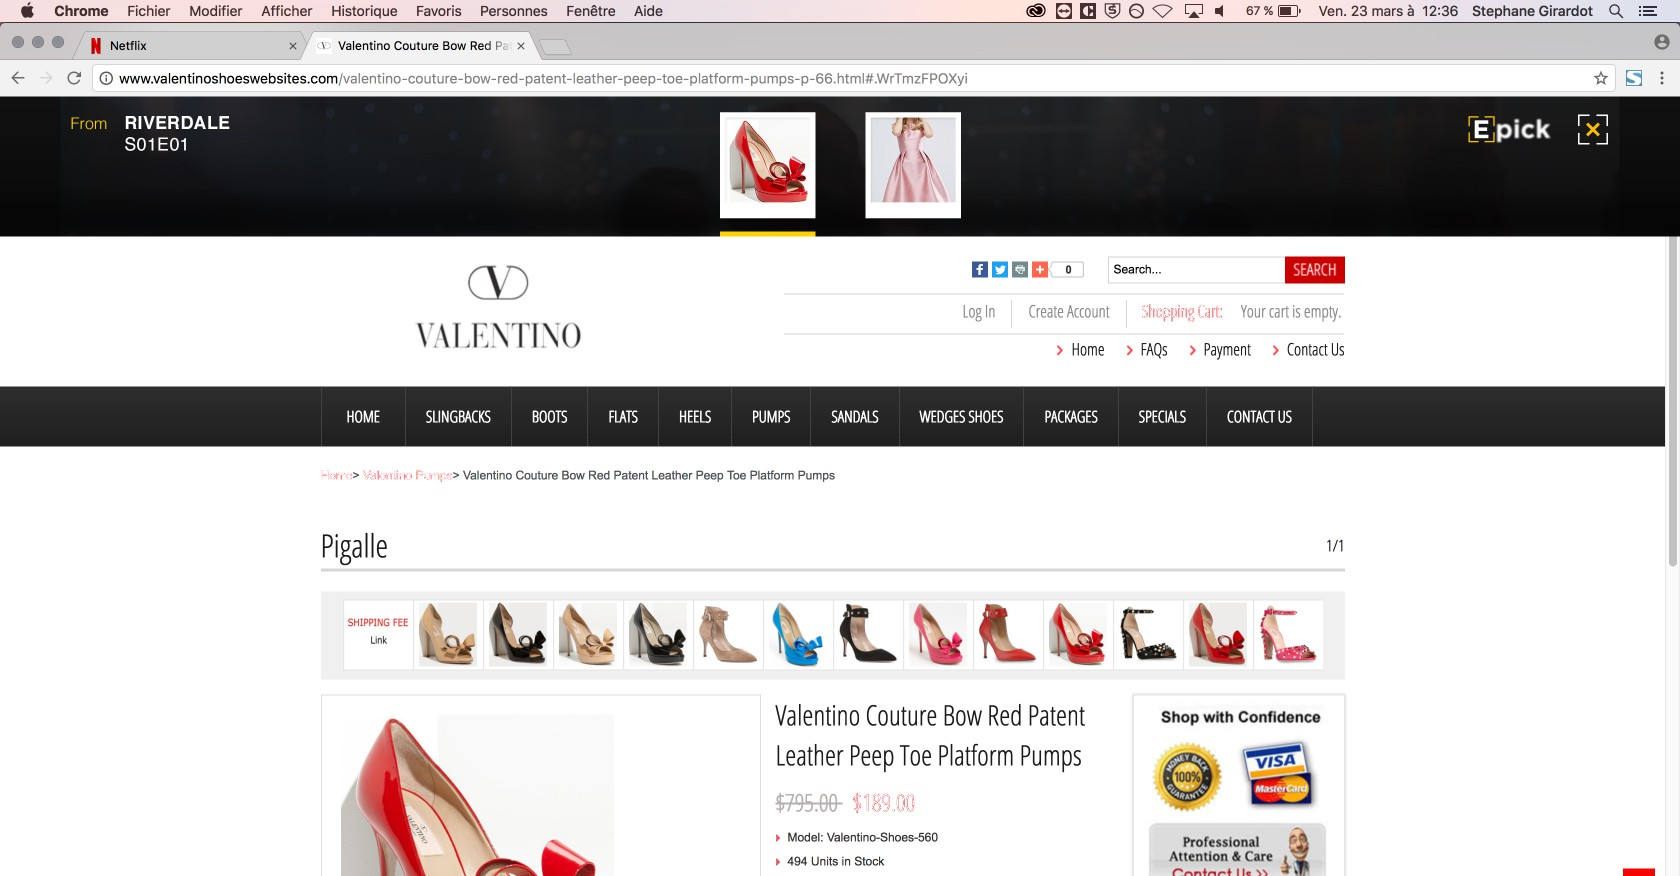
\includegraphics[height=3.8cm]{images/Steps_12.jpg}}
 
  \caption{StoryBoard dessiné par l'agence Ogilvy}
  \label{fig:gallerie1}
\end{figure}
Au final, l’utilisateur est redirigé sur un nouvel onglet vers l’URL du produit dans l'E-shop et un bandeau horizontal rappelle sur quel épisode ce produit a été trouvé et l’ensemble de la wishlist en cours[ figure~\ref{fig:J} ].
La volonté de Watiz est de rester discret et de ne pas interférer avec les fonctionnalités du layer Netflix, même lorsque le résumé de l’épisode arrive pendant la pause au bout de 5sec. [ figure~\ref{fig:F} ].

\subsection{Développement technique général}
Le développement technique de la solution générale va reposer sur trois axes principaux : des algorithmes d'AI, un service cloud et une BDD. En effet, le fait de pouvoir retrouver des vêtements en temps réel dans un flux vidéo nécessite tout d'abord d'avoir une architecture cloud performante. Le choix de Watiz s'est posé sur le service AWS qui propose une multitude de services (lamba, sagemaker, ...) orienté deep learning. Les algorithmes de Watiz se divisent en deux parties comme nous l'avons vu dans la section \ref{sec:technologie} page \pageref{sec:technologie}. Ces algorithmes doivent être rapides et performants. Pour cela, Watiz s'appuie sur ces partenariats avec la recherche pour développer les algorithmes les plus performants possibles. Enfin, la BDD doit être grande et diversifiée afin d'avoir des réponses cohérentes, mais ceci pose des problèmes de temps de calcul pour la recherche de vêtements similaires. Watiz travaille alors sur une parallélisation de ces algorithmes pour être encore plus robuste et pouvoir traiter le flux en temps réel.

\subsection{Développement technique particulier}
Après m'être intéressé à l'usage général et particulier, je me suis mis au travail. À mon arrivée, le projet était déjà en cours. Pour développer cette solution, Watiz a choisi de créer une extension sur Chrome. J’ai donc participé à développer certaines fonctionnalités de l'extension. J’ai commencé tout d'abord à télécharger le projet depuis le repository dans le GitLab et à lire le code afin d'en comprendre la globalité, les différentes fonctionnalités et l’ensemble de ses fonctions. Pour cela, il fallait comprendre d’abord comment fonctionne une extension. J’ai donc activé le mode développeur dans mon browser dans les paramètres de Chrome pour pouvoir y charger notre extension. Ensuite, j’ai lu les configurations de l’extension.\\

Le point de départ de la création d'une extension est la création d'un fichier manifest.json à la racine de notre dossier. Il contient toutes les informations concernant la configuration de l'extension comme le nom, la description et les scripts à charger, et ensuite les permissions (par défaut l’extension est dans une sorte de bac à sable et n'aura accès à rien). Mais dans notre cas, nous souhaitons créer une extension capable de communiquer avec des pages Web, ou avec certaines API du navigateur. Il faut alors préciser dans notre configuration quelles permissions nous souhaitons obtenir (ces permissions seront demandées lors de l'installation de l'extension). Ces permissions peuvent prendre deux formes :
\begin{itemize}
\item Une chaîne de caractères représentant un type de permission en particulier, par exemple l'accès aux onglets tabs (liste des permissions).
\item Un motif représentant un format d'URL auquel on va accéder (Match Patterns).\\
\end{itemize} 

Dans notre cas, nous voulons que notre extension ne fonctionne que sur Netflix. J’ai donc mis en permission ["*://www.netflix.com/watch/*] qui me permet d’autoriser le fonctionnement de l’extension sur Netflix en HTTP ou HTTPS,[*://] sur le visionnage de la vidéo [/watch] quelque soit l’utilisateur et quelque soit la video [/*].\\
La gestion des évènements dans le Manifest.json se fait grâce à la fonction “Background”. Dans notre cas, ce fichier Background.js est enregistré dans le manifeste sous le champ "Background". Ce fichier nous permet d’écouter les actions d’un internaute ayant installé l’extension. Pour cela, nous avons mis deux listener:
\begin{itemize}
\item \textbf{onUpdated}: Cette fonction va nous permettre d’écouter le comportement de l’utilisateur dans le navigateur Chrome. En effet, lorsque l'utilisateur accède à une nouvelle URL dans un onglet, il génère généralement plusieurs événements onUpdated en fonction des diverses propriétés des onglets. Dans notre cas, nous allons nous intéresser à la variable changeinfo et plus particulièrement à sa propriété status lors du chargement de l’URL et de la page.  La propriété “status” va passer par "loading" et "complete". Dès qu’on a un status "complete", on  va appeler le script interact.js qui va lancer le fonction démarrage et qui va vérifier si on est bien sur Netflix sur la série Riverdale épisode 1 pour appeler la fonction init().
\item \textbf{onMessage} : on a utilisé Message Passing (chrome.runtime.sendMessage) qui va écouter les différents messages reçus et qui va répondre en préparant les réponses aux requêtes HTTP. 
La première partie de mon travail, au délà de préparer l’extension comme nous venons de le voir, a été de compléter, nettoyer, simplifier et de segmenter le premier code qui avait été produit. Une grande partie de ce travail s’est faite dans le fichier Interact.js qui, chronologiquement, est lancé par background.js. 
La première problématique à laquelle j’ai répondu est le fait de travailler uniquement sur la vidéo de la série Netflix et non pas sur la totalité du player. En effet, si on regarde [ figure~\ref{fig:4.2.1} ] et [ figure~\ref{fig:4.2.2} ] on voit qu’à aucun moment, un div nous donne exactement la dimension de la vidéo. \\
\end{itemize} 
\begin{figure}[!ht]
\begin{center}
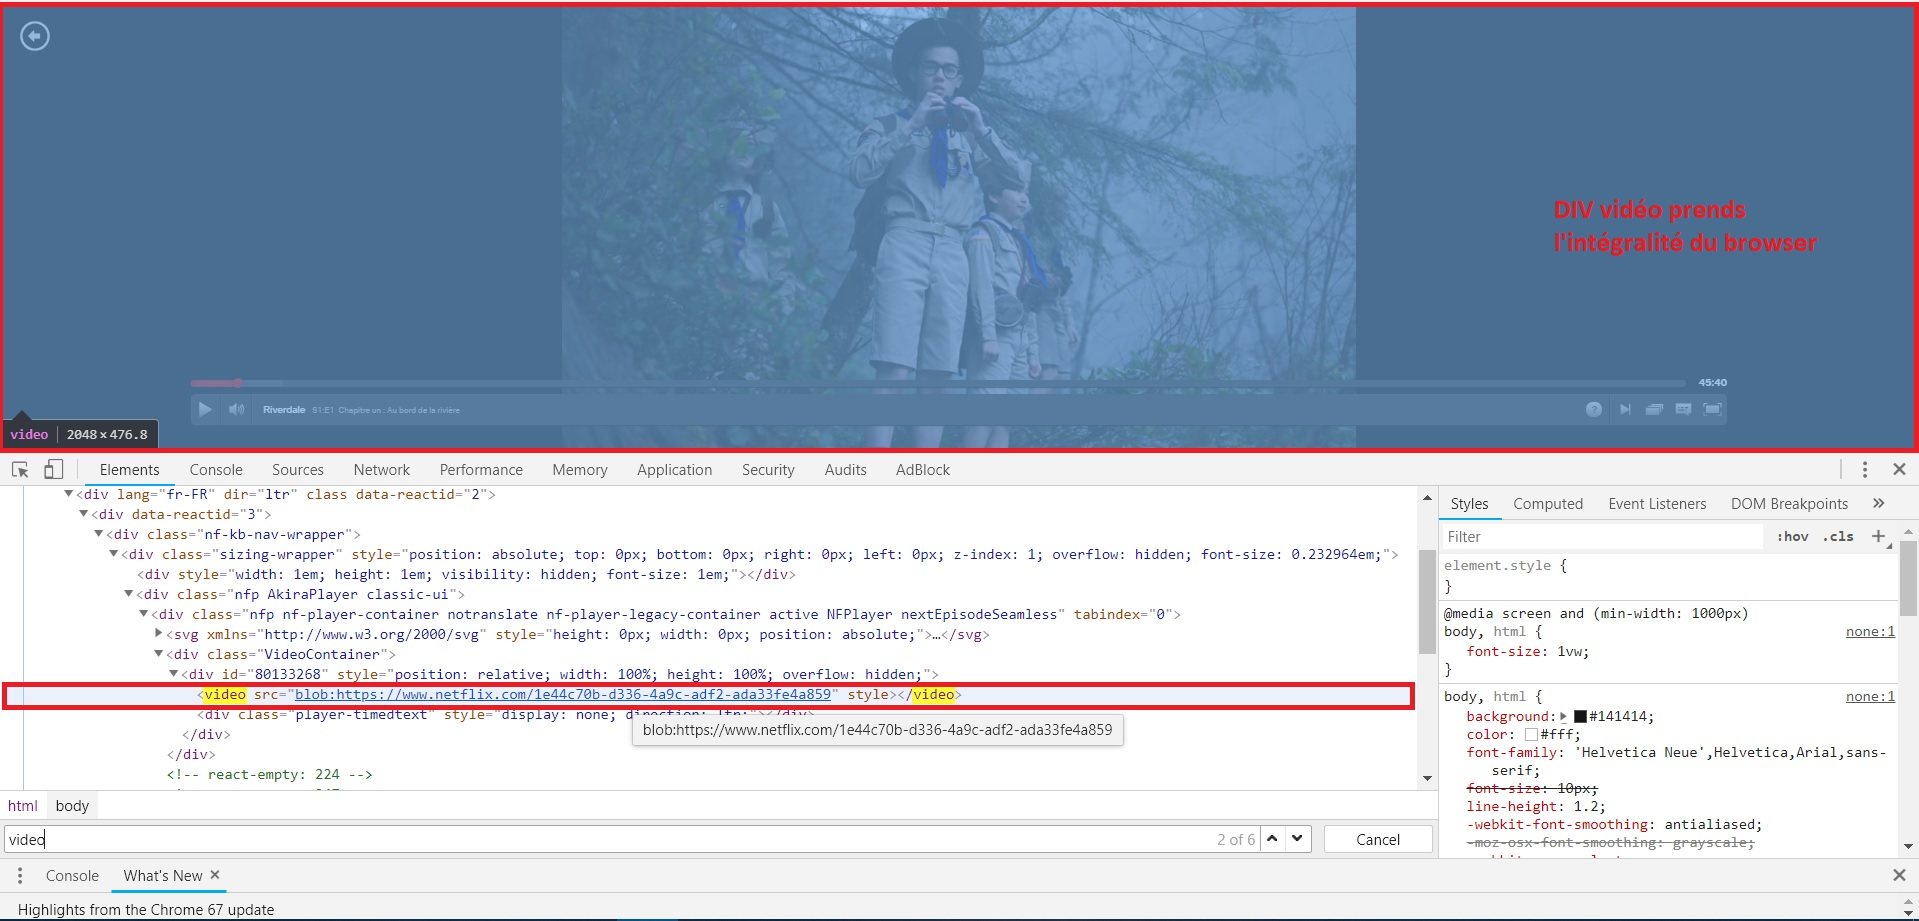
\includegraphics[height=7cm]{images/video.jpg}
\caption{La balise video prend tout l'espace de navigateur}
\label{fig:4.2.1}
\end{center}
\end{figure}

\pagebreak
\newpage
\begin{figure}[!ht]
\begin{center}
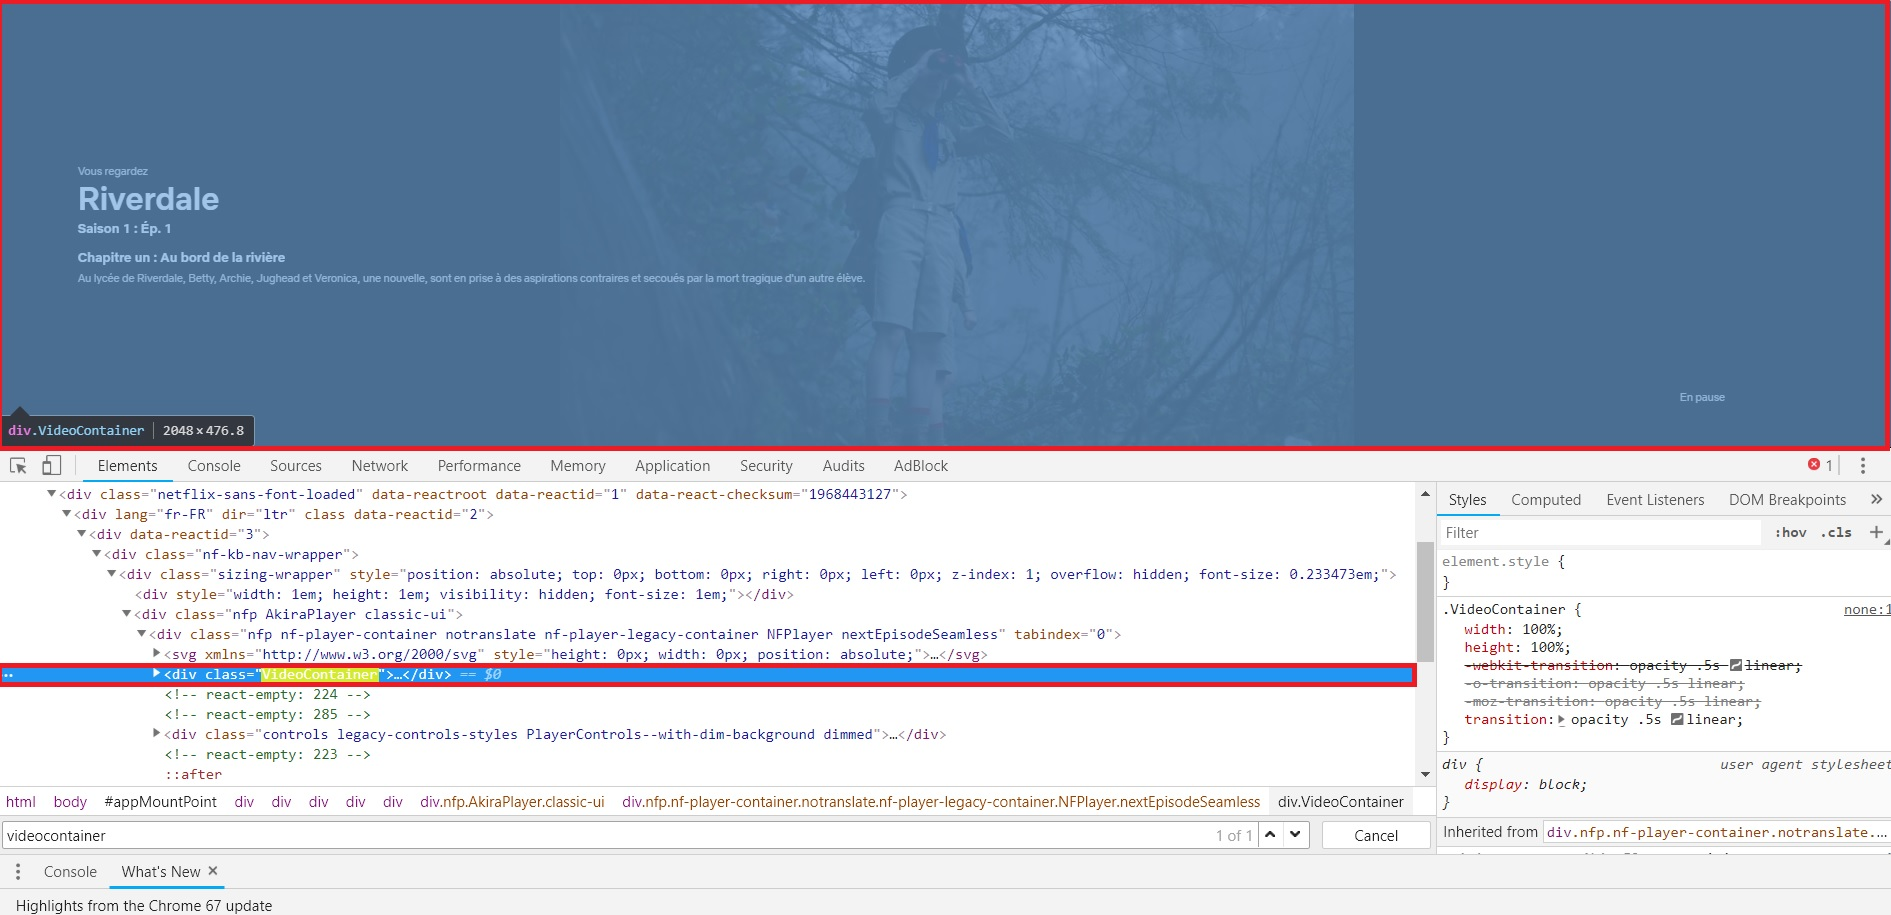
\includegraphics[height=7cm]{images/Videocontainer.jpg}
\caption{La balise div videocontainer prend tout l'espace de navigateur}
\label{fig:4.2.2}
\end{center}
\end{figure}
De ce fait, pour introduire tous nos visuels (UI, wishlist présenté à la section~\ref{AN}, page~\pageref{AN}), j’ai dû créer un container de la taille de la vidéo Netflix.\\
Dans la fonction init(), j'ai effectué des calculs pour créer un container qui ait les mêmes dimensions que la video de Netflix. C'est dans ce container que l'on mettra tous nos composants comme le logo de l'extension, le panier qui va contenir tous les vêtements choisis ou encore les "BOX" cliquables sur les vêtements.
Pour cela, il fallait prendre en compte la taille de la vidéo qui a un ratio de 16/9 . Le player de Netflix garde ce ratio en ajoutant des bandeaux noir horizontalement (à gauche et à droite) ou verticalement (en haut et en bas) de la vidéo. Ces bandeaux noirs sont en rapport avec le ratio de la vidéo et le ratio du navigateur. Considérons qu'un ratio est la division de la largeur par la hauteur (R=Largeur/Hauteur). Si le Ratio du Navigateur est inférieur au Ratio de la vidéo, alors les bandeaux seront en haut et en bas. À l'inverse, les bandeaux seront à gauche et à droite. 
Pour garder la ratio (16/9 =1.7778), j’ai calculé la taille des bandeaux noirs pour garder notre container sur la vidéo quand on a un ratio supérieur ou inférieur à 1.7778 [ figure~\ref{fig:4.4} ] :\\
\begin{figure}[!ht]
\begin{center}
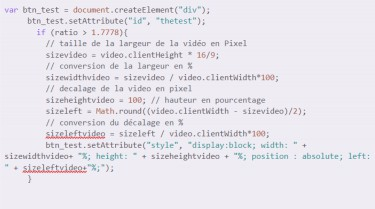
\includegraphics[height=5.5cm]{images/codeJavaScript1.jpg}
\caption{Une partie de code JavaScript pour le calcul }
\label{fig:4.4}
\end{center}
\end{figure}
\pagebreak
\newpage
Pour aller plus loin, j'ai utilisé la fonction  onresize pour s'adapter aux différentes tailles d’écran. En effet, lorsqu’un utilisateur va changer la taille de son navigateur, la taille de la vidéo et du player vont changer. Il faut donc également adapter la taille de mon Div. J’ai donc repris les mêmes calculs dans la fonction windows.resize.\\
La deuxième problématique abordée concerne l’apparition des visuels Epick. Comme expliqué dans la section \ref{CP}, la solution Epick n'apparaît que lorsque le player est en pause. Il a fallu donc mettre un listener sur cette fonctionnalité qui écoute le statut de la vidéo (s’il est en pause ou en play mode).
Cette problématique n'était pas facile car la pause peut s'effectuer de deux manières différentes (clic sur le bouton pause dans le player ou enfoncement de la barre d'espace). Cette fonctionnalité était déjà implémentée dans l'ancien code comme suit:
\begin{itemize}
\item Un listener sur le bouton pause du player  
\begin{figure}[!ht]
\begin{center}
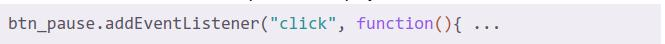
\includegraphics[height=0.9cm]{images/1.jpg}
\end{center}
\end{figure}
\item Un listener sur la barre d'espace 
\begin{figure}[!ht]
\begin{center}
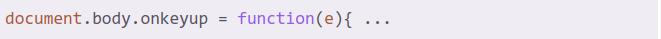
\includegraphics[height=0.8cm]{images/2.jpg}
\end{center}
\end{figure}
\end{itemize} 
J'ai noté l'apparition d'erreur lorsque l'on alternait le lancement de la pause (opérations successives entre le fait d'appuyer sur pause ou d'utiliser la barre d'espace). La principale erreur était la disparition du panier et des box.
Pour résoudre ces bugs, j’ai utilisé une fonction de JavaScript qui traite cette problématique  en même temps (\textit{onpause} et \textit{onplay}) sur un div particulier. J’ai donc récupéré ma variable “video” avec \textit{document.getElementByTagName} et ensuite utilisé le video.onpause et vidéo.onplay. 
Ceci m’a permis de régler le problème et de réduire le nombre de lignes jusqu'à 20 (il en comprenait 100 à l'origine).\\

Ces deux problématiques m’ont permis de comprendre plus finement le code et de travailler sur du JavaScript native. Le projet est toujours en cours et il me reste encore des tâches de nettoyage et de segmentation du code pour arriver à la fin à un POC Epick stable. Ensuite viendra la nouvelle version du code pour brancher les algorithmes à l’extension.\\
%%%%%%%%%%%%%%%%%%%%%%%%%%%%%%%%%%%%%%%%%%%%%%%%%%%%%%%%%%%%%%%%%
\subsection{Développer les deux pages du projet Epick}
Au cours de mon travail sur le projet Epick, j'avais pour mission de créer deux pages web pour télécharger l’extension Chrome.
Ogilvy nous a envoyé le design et la maquette de ces deux pages [ figure~\ref{fig:4.5} et~\ref{fig:4.6} ].\\
\begin{figure}[t]
\begin{minipage}{0.5\linewidth}
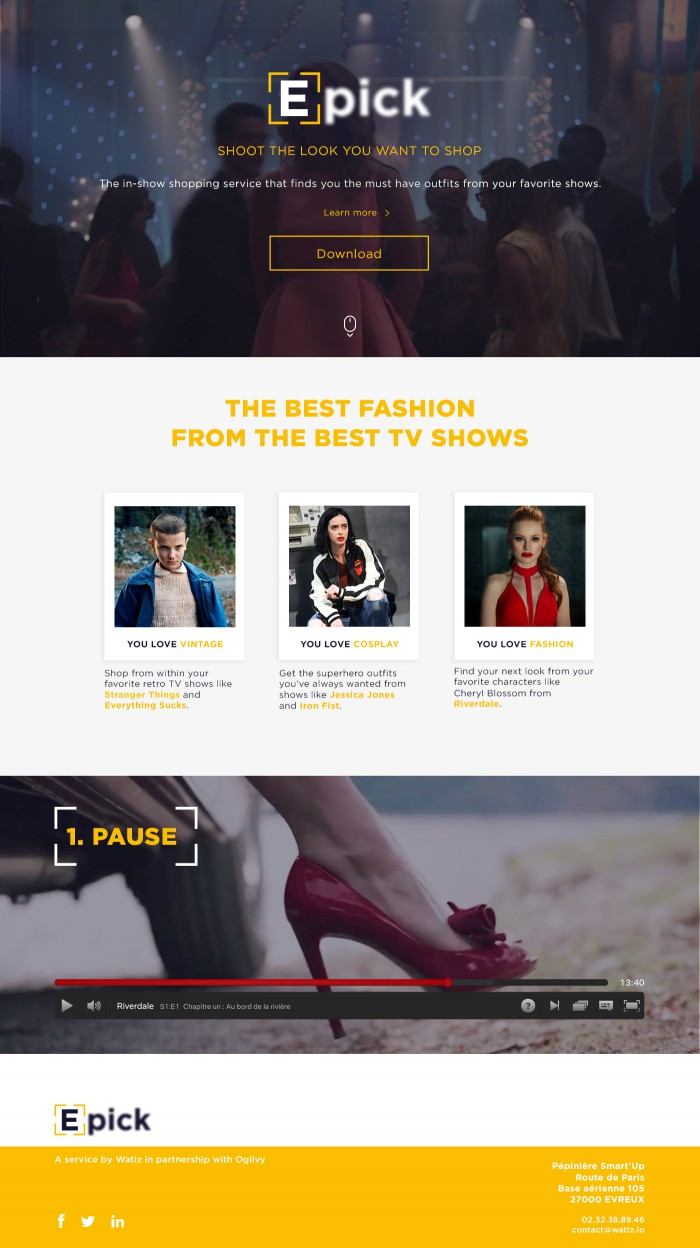
\includegraphics[height=13cm]{images/Epick_Landing_page.jpg}
\caption{Landing page}
\label{fig:4.5}
\end{minipage}\hfill
%%%%%%%%%%%
\begin{minipage}{0.45\textwidth}
Cette démarche a été très intéressante en tant que développeur web front-end car j'étais confronté à un besoin client et à un design créé par un designer.
J'étais dans l'obligation de respecter le design (couleur, font, taille, positionnement des éléments).
J’ai commencé par définir la structure de la première page (Landing page [ figure~\ref{fig:4.5}]) en HTML. Dans ma méthodologie, pour chaque élément HTML que je créais, je créais un style CSS associé. J'ai également choisi d'utiliser la librairie Boostrap afin de faciliter mon développement et qui, de plus, est très pratique pour la responsivité du design.
Une fois fini le code HTML et CSS de la page "Landing", j'y ai ajouté des fonctionnalités en utilisant JavaScript et Jquery.
Le bouton "Download" permet de télécharger l'extension Epick. L’icône de souris permet de scroller la page jusqu'à la vidéo qui explique la fonctionnalité de l'extension.\\
\linebreak
\end{minipage}
\end{figure}

\begin{figure}[!htbp]
\begin{minipage}{0.46\linewidth}
La page "Welcome" apparaîtra après avoir téléchargé l'extension Epick et proposera aux internautes des liens vers certains moments de l’épisode 1 de la série Riverdale où il y a des vêtements déjà identifiés. J'ai donc copié/collé le code de la page "Landing" et je l'ai modifié.
Dans la rubrique QUICK PICKS, il a fallu faire un changement d'aspect des photos au survol de la souris. Le hover sur les photos avec la souris remplacera les photos par d'autres photos (regardez la deuxième photo dans le rubrique QUICK PICKS de figure~\ref{fig:4.6}).

\end{minipage}\hfil
\begin{minipage}{0.35\linewidth}
    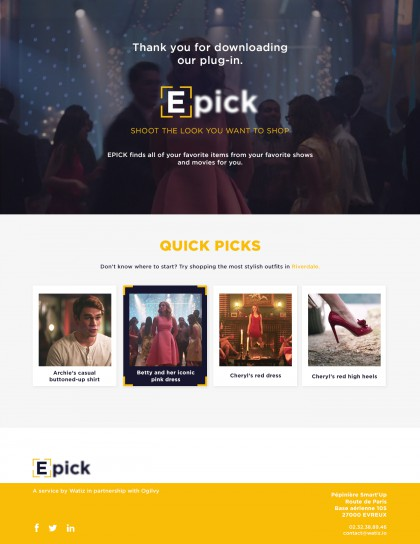
\includegraphics[height=8cm]{images/Epick_Welcome_page_preview.jpg}
    \caption{Welcome page}
 \label{fig:4.6}
\end{minipage}
\end{figure}
%%%%%%%%%%%%%%%%%%%%%%%%%%%%%%%%%%%%%%%%%%%%%%%%%%%%%%%%%%%%%%%%%%
\newpage
\subsection{Amélioration et généralisation du POC Epick }
Le projet Epick est toujours en cours. Pour généraliser la solution à d'autres sites, il reste encore beaucoup de travail et jusqu'à la fin de mon stage, je vais me concentrer sur les tâches suivantes :
\begin{itemize}
\item \textbf{}Nettoyer et structurer le code.
\item \textbf{}Finir les corrections.
\item \textbf{}Faire connecter l'extension avec l'algorithme du détecteur.
\end{itemize} 
\newpage
%%%%%%%%%%%%%%%%%%%%%%%%%%%%%%%%%%%%%%%%%%%%%%%%%%%%%%%%%%%%%%%%%%%%%%%%%%%%%%%%%%%%
\section{Développer le site de la société Watiz}
\subsection{Présentation de l’existant}
\begin{wrapfigure}{R}{0.44\textwidth}
\captionsetup{font=small}
\centering
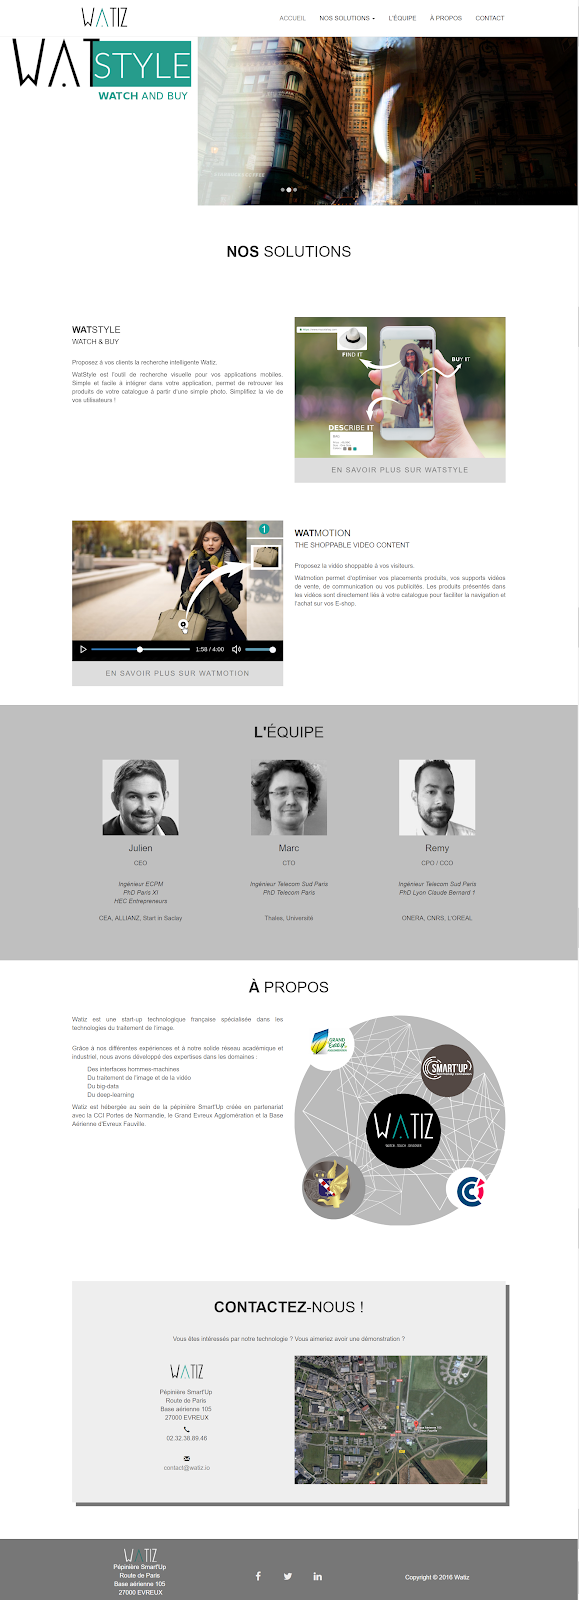
\includegraphics[height=18cm]{images/Watiz_WebSite_Home.png}
\caption{\label{fig:4.7}ScreenShot de l'ancien site.}
\end{wrapfigure}
Ce site a été réalisé en interne[ figure~\ref{fig:4.7} ].
Au niveau programmation, il s’agit d’un site statique composée de trois pages, d’un menu et d’un sous-menu pour la rubrique "Solutions".
Le site se composait de cinq sections. La section "Accueil" était un carrousel de trois images qui représentait l'activité et les solutions de l'entreprise.
La section "Solutions" décrivait les solutions développées à l'époque par Watiz (titre, description et une photo avec un bouton “En savoir plus” qui ouvrait une page dédiée à chaque produit).
Les sections "Equipe" et "A propos" présentaient l'équipe et l’entreprise ainsi que les différents partenaires de l'entreprise.
La section "Contactez-nous" était une section de localisation avec une image de carte et les coordonnées postales et digitales de l'entreprise. On trouvait ensuite le "Footer" avec le rappel des coordonnées et des liens vers les réseaux sociaux : LinkedIn, Facebook et Twitter.
\subsection{Critiques de l’existant}
Le site web de Watiz n'était plus à jour et son design commençait à vieillir (par exemple, Watiz a décidé de ne plus communiquer sur son service WatMotion). 
Au niveau du contenu, Watiz voulait avoir une présentation plus orientée vers l'international et faire apparaître son antenne commerciale localisée en région parisienne. Il était également nécessaire d'améliorer et/ou d'ajouter des descriptions pour favoriser la compréhension des internautes. 
D'un point de vue visuel, le site web était trop simple et les photos n'étaient pas représentatives de leurs activités et ne captaient pas l'attention des internautes.
Pour la rubrique "Contactez-nous", l'absence de formulaire dans le site ne facilitait pas à la prise de contact.\\

\newpage
De plus, le site web ne jouait pas sur les différences de couleur pour inviter l'internaute à interagir avec les différentes rubriques ou boutons (la couleur dominante était le gris) et il n'utilisait pas d'effet de surbrillance ou de coloration de boutons.
\subsection{Objectifs de la mise à jour du site (analyse des besoins)}
Watiz avait besoin d’un nouveau site qui :
\begin{itemize}
\item \textbf{} Présente les solutions actuelles de l'entreprise.
\item \textbf{} Possède un design adapté plus moderne et facilite la mise en avant du contenu. 
\item \textbf{} Soit simple et compréhensible permettant d'obtenir des informations en quelques clics.
\item \textbf{} Soit compétitif visuellement avec les sites des concurrents. 
\item \textbf{} Soit réalisable en quelques semaines afin d'être mis en ligne avant l'événement Vivatechnology.
\end{itemize} 
\subsection{Proposition}
Un site efficace doit se baser sur trois aspects. Premièrement, celui-ci doit réussir à être accessible et visible pour sa cible. En effet, l’un des premiers enjeux est de réussir à acheminer du trafic sur le site en question. 
Le site doit aussi répondre au besoin de sa cible, il doit donc être clair et pensé pour que l’utilisateur puisse y trouver son compte, que cela soit pour chercher une information ou acheter un produit. Un site qui ne satisfait pas ses visiteurs n’est pas efficace !\\
Enfin, le site doit savoir faire revenir ses visiteurs et fédérer une communauté de visiteurs réguliers. Un site qui ne fidélise pas ses visiteurs n’est pas pertinent !
A partir de ces observations, j'ai commencé à rédiger un rapport pour présenter mes propositions en justifiant mes choix. Pour cela il fallait :
\begin{itemize}
\item \textbf{}Faire une veille concurrentielle et tendancielle en regardant les sites à la mode et les sites des principaux acteurs du secteur.
\item \textbf{}Regarder quelles sont les tendances Web Design en 2018.
\item \textbf{}Faire un état de l'art sur les bonnes méthodes UX/UI.
\item \textbf{}Faire un story board par Photoshop pour le nouveau site.\\
\end{itemize} 
Ma proposition consistait à :
\begin{itemize}
\item \textbf{}Garder la même structure que le site existant afin d'utiliser le même template.
\item \textbf{}Insérer une vidéo dans la page d'accueil avec une surcouche noire d'opacité proche de zéro, et au milieu de la vidéo, le logo de Watiz avec une phrase d’accroche. L'idée était de mettre une vidéo de promotion de la société pour capter tout de suite l'intérêt de l'internaute.
\item \textbf{}Ajouter une section pour présenter les avantages des produits Watiz et une autre section pour la technologie.
\item \textbf{}Ajouter des Google Maps pour chacun des deux sites avec leurs coordonnées (email, téléphone...) afin de simplifier leurs localisations.
\item \textbf{}Ajouter un  formulaire de contact pour encourager les internautes à envoyer un message facilement.
\item \textbf{}Créer des pages dédiées à chaque rubrique accessible par des boutons "En savoir plus" 
\item \textbf{}Ajouter pour chacune des solutions un démonstrateur ou une vidéo de démonstration et une section "Comment ça marche".
\item \textbf{}Utiliser davantage la couleur verte (déjà présente dans le logo) et peut-être un usage léger du bleu.  
\end{itemize} 

\subsection{La maquette (Storyboard)}\label{subsec:MA}
\begin{wrapfigure}{R}{0.45\textwidth}
\captionsetup{font=small}
\centering
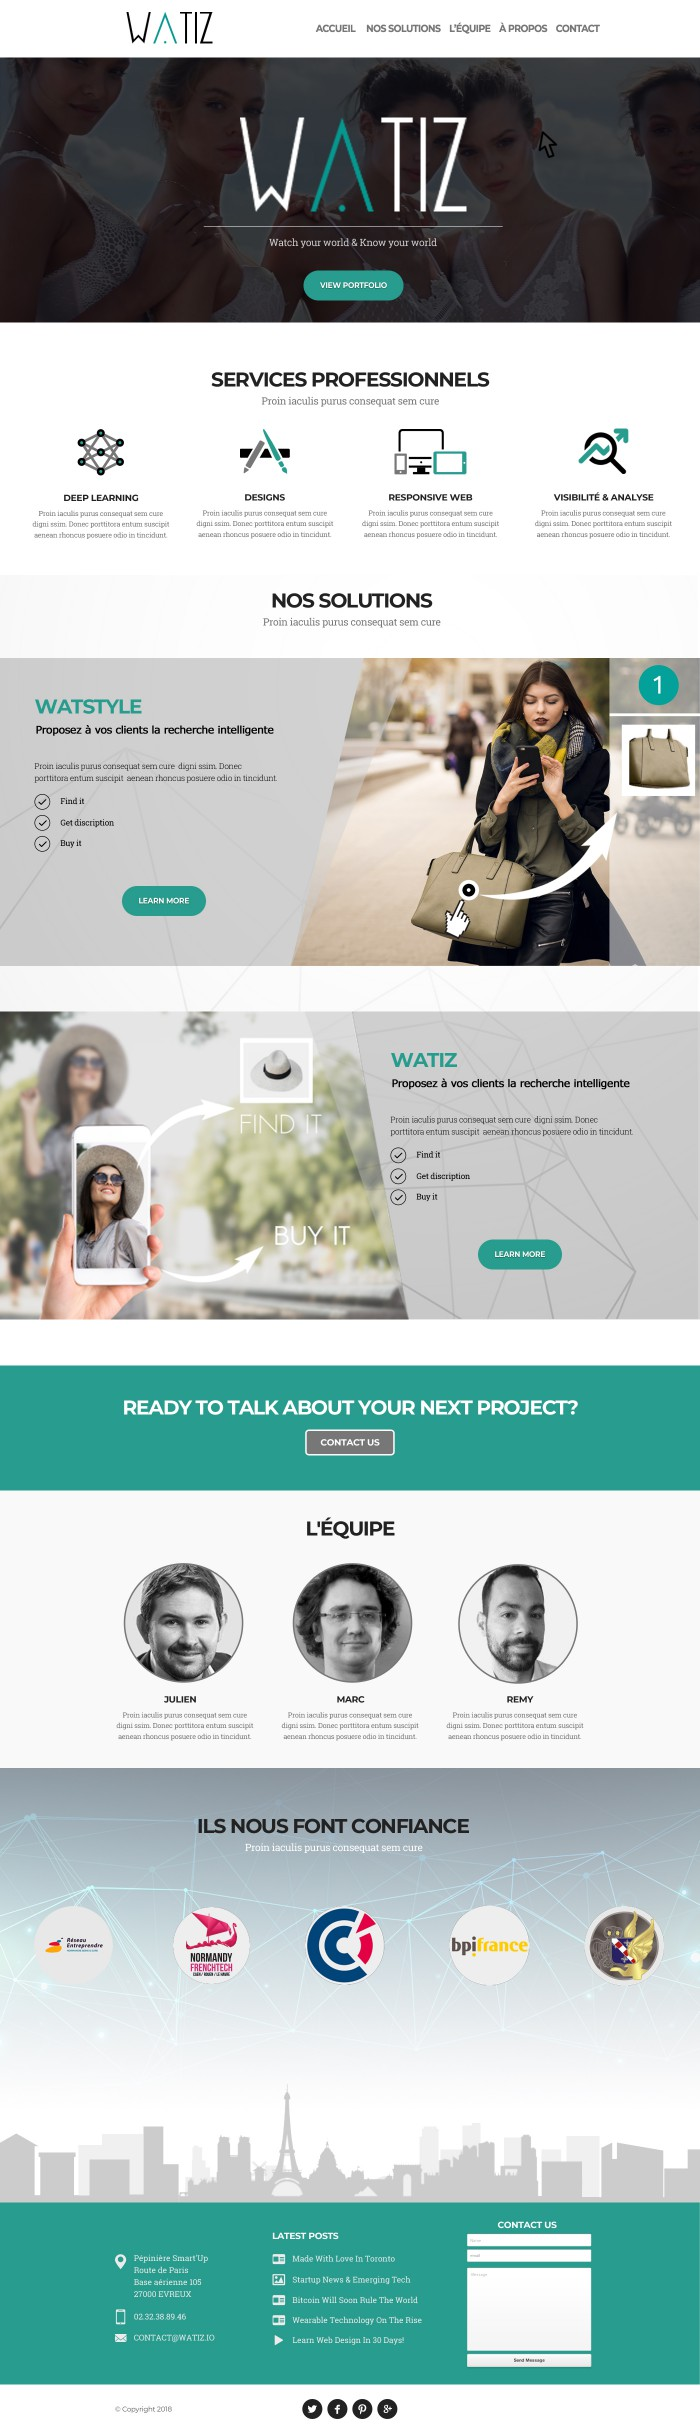
\includegraphics[height=17.5cm]{images/StoryBoard1.jpg}
\caption{\label{fig:4.8}Prémiere Storyboard.}
\end{wrapfigure}
Une maquette est l’équivalent d’un site web en version imprimée \cite{3}. La création d’une maquette intervient souvent après l’étude des besoins du client (la société Watiz) et l’élaboration d’un cahier des charges.
En général, elle est réalisée par un graphiste qui maîtrise les outils de PAO et qui a de bonnes connaissances en design pour le Web. Elle peut aussi être réalisée par les designers d’interface (UI designer). Les outils les plus connus sont Photoshop, InDesign ou Sketch.\\
Ayant une facilité pour le design et maîtrisant bien le photoshop, je me suis permis de réaliser la maquette par moi même. J’ai donc utilisé une grille qui est organisée en lignes horizontales et en lignes verticales, qui rend les contenus plus lisibles et plus structurés. Elle m'a permis également d’adapter les contenus aux différentes tailles d’écran, et donc de penser responsive. Le fait d'avoir un esprit créatif pour le design en plus de mes compétences front-end, Watiz a pu économiser du temps et/ou de l'argent dans l'élaboration de la maquette du site.

\subsection{Cahier des charges}
Un cahier des charges est un document qui liste les besoins du client ainsi que les différentes étapes de réalisation jusqu’à la mise en ligne finale. Il est extrêmement important d’en avoir un pour être certain que l’entreprise et moi partageons les mêmes objectifs.
Après avoir rendu mon rapport, mon tuteur a accepté presque toutes mes propositions, sauf ce qui concerne une vidéo promo. Donc nous avons écrit ensemble le cahier des charges. Voici un résumé des constraintes présentes dans le cahier des charges :\\
%%%%%%%%%%%%%%%%%%%%%%%%%%%%%%%%%%%%%%%%%%%%%%%%%%%%%%%%%%%%%%%%%%%%%%%%%%%%%%%%%%%%
\newpage
\begin{enumerate}
\item Nous gardons le même template que le website actuel et la même technique de scrolling page.
\item Il faut changer tous les visuels du site et nous allons utiliser des icônes pour présenter facilement les avantages et la technologie.
\item Pour le haut de page, nous utiliserons une image ou bien un carrousel. 
\item Pour la  charte graphique, les couleurs retenues sont le blanc, le noir, le gris et le vert. 
\item Pour la famille de polices, nous utiliserons : Abel|Anton|Muli|Pacifico|Varela.
\item Le site sera rédigé dans un premier temps en anglais, la version française sera développée dans un deuxième temps.
\item Un formulaire de contact sera présent et sera codé sans back-end en JavaScript.
\item Le website doit être responsive pour s’adapter à toutes les tailles d’écran (PC, Netbook, Tablette, Mobile). 
\item Le site doit être téléchargé sur GitLab et mis en ligne sur le serveur OVH avant le 24 mai 2018.
\end{enumerate} 

\subsection{Développement}
\begin{figure}[!htbp]
\centering
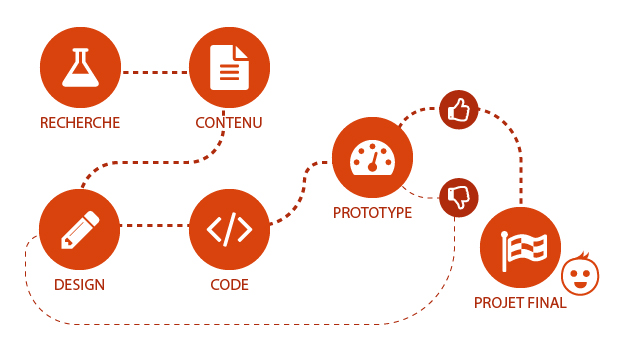
\includegraphics[height=7cm]{images/developement.png}
\caption{Les différents étapes pour réaliser le site web}
\label{fig:4.9}
\end{figure}

Après avoir mis en place le cahier des charges à partir de la recherche, de l'élaboration du contenu et du design (la maquette story bord), je suis arrivé à l'étape du développement [figure \ref{fig:4.9}] dans les délais imposés. 
La maquette est le point de départ de tout intégrateur. En effet, mon premier travail était de traduire la maquette en langage web, c’est à dire en HTML, CSS et JS \cite{4}. Ayant été le graphiste, je connaissais déjà les éléments interactifs qui nécessitaient du Javascript. Donc, j’ai d’abord mis en place la structure général du HTML.\\
Dans le head, j’ai ajouté les métadonnées qui permettent aux réseaux sociaux de mieux comprendre le contenu de la page et d’afficher le contenu que l’on souhaite et le meta Viewport pour que l'affichage occupe tout l'espace disponible avec une taille de 100\%. Il y a aussi le titre du document avec l'icône qui apparaîtra dans l’onglet et les références aux feuilles de style utilisées par le document et le framework bootstrap \cite{5}.\\
En revanche, je n’ai pas mis les références aux javascripts utilisés par le document dans le header mais à la fin du body pour une question de performance. En effet, le traitement d'une page web par un navigateur est séquentiel de haut en bas. Placer les scripts au plus bas permet de charger les éléments importants de la page web.
J’ai organisé la page index.html selon l'organisation en groupes de calques du fichier Photoshop. Leurs noms sont écrits sous forme de commentaires HTML et cela m’a aidé à ajouter de manière organisée des balises HTML qui affichent le contenu.
Chacun de ces groupes d'éléments constituant une sorte de grande partie, j’ai utilisé la balise HTML5 <section>. J’y ai ajouté un id reprenant le nom qui est dans mon commentaire, ce qui  m’assure une organisation  de mon CSS adéquate.\\

Le menu a été paramétré de façon à ce qu’il s’affiche parfaitement dans la page : la largeur du menu a été ajustée, le texte de chaque onglet a été centré, les couleurs ont été modifiées pour qu’elles soient en accord avec celles du site.
J'ai utilisé le bootstrap qui comporte un système de grille simple et efficace pour mettre en ordre l'aspect visuel de page web. Il apporte du style pour les boutons, les formulaires, la navigation, etc.. Il m’a permis ainsi de concevoir le site web rapidement et avec peu de lignes de code ajoutées.\\

La grille de Bootstrap étant responsive, elle s'adapte à toutes les dimensions d'écran. En fait, elle reprend le concept de breaking-points qui sont en général 4 breaking-points :
\begin{itemize}
\item \textbf{Les très petits écrans} (< 768 px, pour les écrans dont la largeur est comprise entre 0 px et 768 px).
\item \textbf{Tablettes} (768 px - 991 px).
\item \textbf{Ordinateurs} (992 px - 1199 px).
\item \textbf{Grands écrans} d'ordinateurs et télévisions.\\
\end{itemize}
A partir des breaking-points, j’ai contrôlé tous les éléments de pages et les ai rendus responsive en utilisant @media queries qui définit les techniques pour l'application de feuilles de styles en fonction des périphériques de consultation utilisés pour du HTML.\\
En ce qui concerne la section “Contact Us”, j’ai fait deux lignes. La première que j’ai divisée en deux colonnes, et dans chacune de ces colonnes, j’y ai mis un div canvas pour les cartes google maps que j’ai codées en JavaScript \cite{6} dans le fichier mapScript. Pour cela, j’ai d’abord déclaré les markersData variables et j’ai ensuite initialisé deux variables avec les Coordonnées de deux sites (Evreux, Arcueil) . 
Dans la deuxième ligne, j’ai fait une seule colonne où j’ai mis un bouton animé qui permet d’afficher le formulaire de contact.\\
L’affichage de ce formulaire a été fait avec JavaScript dans un fichier unique. J’ai utilisé la bibliothèque Jquery \cite{7} pour le développement de JavaScript et mis en place des fonctions pour la validation des champs et pour la vérification de la syntaxe email.\\

Comme demandé dans le cahier des charges, il n’y a pas de back-end et j’ai réalisé ce formulaire avec un service de Google, Google App Mail \cite{8}, qui permet d'envoyer un email à partir d'une page HTML "statique" sans  avoir un serveur.

Google App Mail a comme avantages :
\begin{itemize}
\item De ne pas avoir  de "Backend" à déployer / maintenir.
\item D’être entièrement Customisable.
\item D’envoyer des mails par l'intermédiaire de Google Mail qui est Whitelisted-Everywhere (grand succès de la délivrabilité).
\item De collecter / stocker toutes les données de formulaire dans une Spreadsheet pour un affichage facile.
\end{itemize}
Le style du site étant particulier, il a fallu modifier le template d’origine. La grille Bootstrap m’a donné une base qui m’a permis d'organiser tous les éléments dans les colonnes, mais elle ne suffit pas à gérer toutes les règles de style. Le fichier Style.css contient tous les styles pour les éléments et les balises Html. J’ai suivi une convention de nomenclature pour  retrouver les éléments à modifier facilement.\\
J’ai utilisé animate.css pour certains éléments. Il s’agit d’une feuille de style qui utilise les animations CCS3. Celles-ci sont obtenues en appliquant des classes CSS définissant ces transitions/animations.
À la fin du body, j’ai déclaré tous les scripts utilisés dans cette page,  la bibliothèque de Jquery et Wow.js, une bibliothèque JavaScript fonctionnant de manière autonome.\\

\textbf{Google analytics} est un service gratuit de Google qui nous permet d’insérer un code dans toutes les pages de notre site Web. Avec ce code, Google cumule des milliers de statistiques sur ce qui se passe sur le site. C’est un service essentiel pour tous les sites Web. Ces statistiques sont accessibles directement à partir du compte Google de l'entreprise Watiz et à n’importe quel moment.\\ 

Une fois la page index terminée, j’ai commencé à développer les pages restantes en suivant la même technique.
Un test technique a été fait avant le téléchargement. J’ai testé le website sur différents navigateurs pour voir comment il réagit et vérifier qu’il n’y ait pas de bugs avec des émulateurs de Google Chrome et de Firefox. Les deux navigateurs embarquent par défaut un émulateur accessible dans les outils de développement (F12). Il permet de choisir différents appareils pour vérifier l'affichage du site et simule également l'agent utilisateur.\\
D’autres outils sont disponibles pour faire ce type de test, comme par exemple :
\begin{itemize}
\item \textbf{Extension Responsive Inspector} qui permet d'afficher les règles\textit{@media}  définies par le site.
\item \textbf{Extension Web Developer} qui permet également, dans le menu Resize, d'afficher les pages à différentes résolutions.\\
\end{itemize} 
Deux jours avant la date de livraison, j’ai pushé la première version (préproduction) sur ma branche sur Gitlab [figure \ref{fig:4.10}] [figure \ref{fig:4.11}]. Ensuite, je l’ai téléchargé vers le serveur OVH pour le tester et avoir les retours de mes collègues sur les supports que l'on souhaite prendre en charge.\\

Suite à ces tests, il y avait encore des modifications et quelques bugs concernant la responsivité du site et le formulaire de "Contact us". J’ai donc corrigé les fautes et je l’ai mis sur le serveur le jour prévu de la livraison.

À présent, \textbf{une nouvelle version} est en cours pour des modifications et améliorations:
\begin{itemize}
\item Sécuriser le formulaire. 
\item Mentions légales. 
\item Bandeaux cookies.
\item Passer serveur sur branche master.
\item Crédits photos.
\item Site en français.
\end{itemize} 
%%%%%%%%%%%%%%%%%%%%%%%%%%%%%%%%%%%%%%%%%%%%%%%%%%%%%%%%%%%%%%%%%%%%%%%%%%%%%%%%%%%%
\begin{figure}[t]
\begin{minipage}{0.5\linewidth}
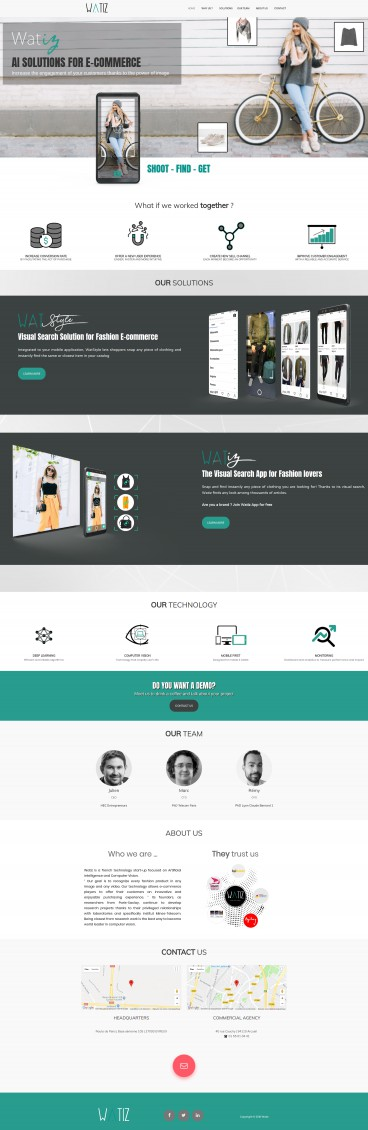
\includegraphics[height=22cm]{images/SiteActuelle.jpg}
\caption{Page d’accueil}
\label{fig:4.10}
\end{minipage}\hfill
%%%%%%%%%%%%%%%%%%%%%%%%%%%%%%%%%%%%%%%
\begin{minipage}{0.45\textwidth}
  \centering
  \subfloat[Page Watiz]{\label{fig:4.11a}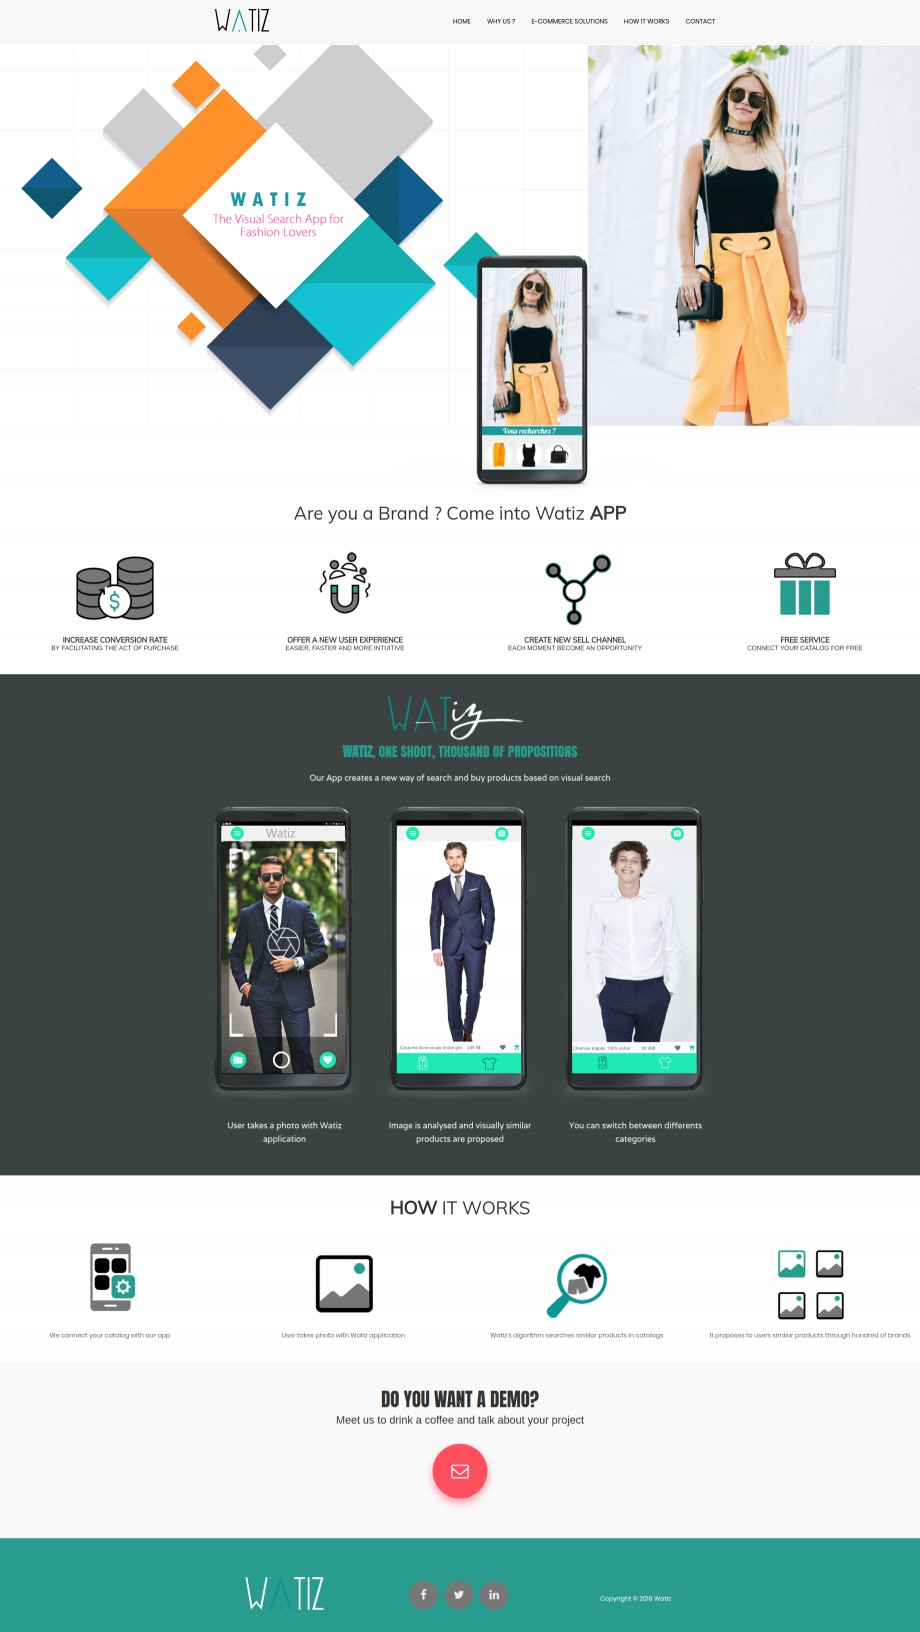
\includegraphics[height=10.2cm]{images/Watiz.jpg}}
  ~\\ %saute une ligne dans la galerie d'image
  \subfloat[Page Watstyle]{\label{fig:4.11b}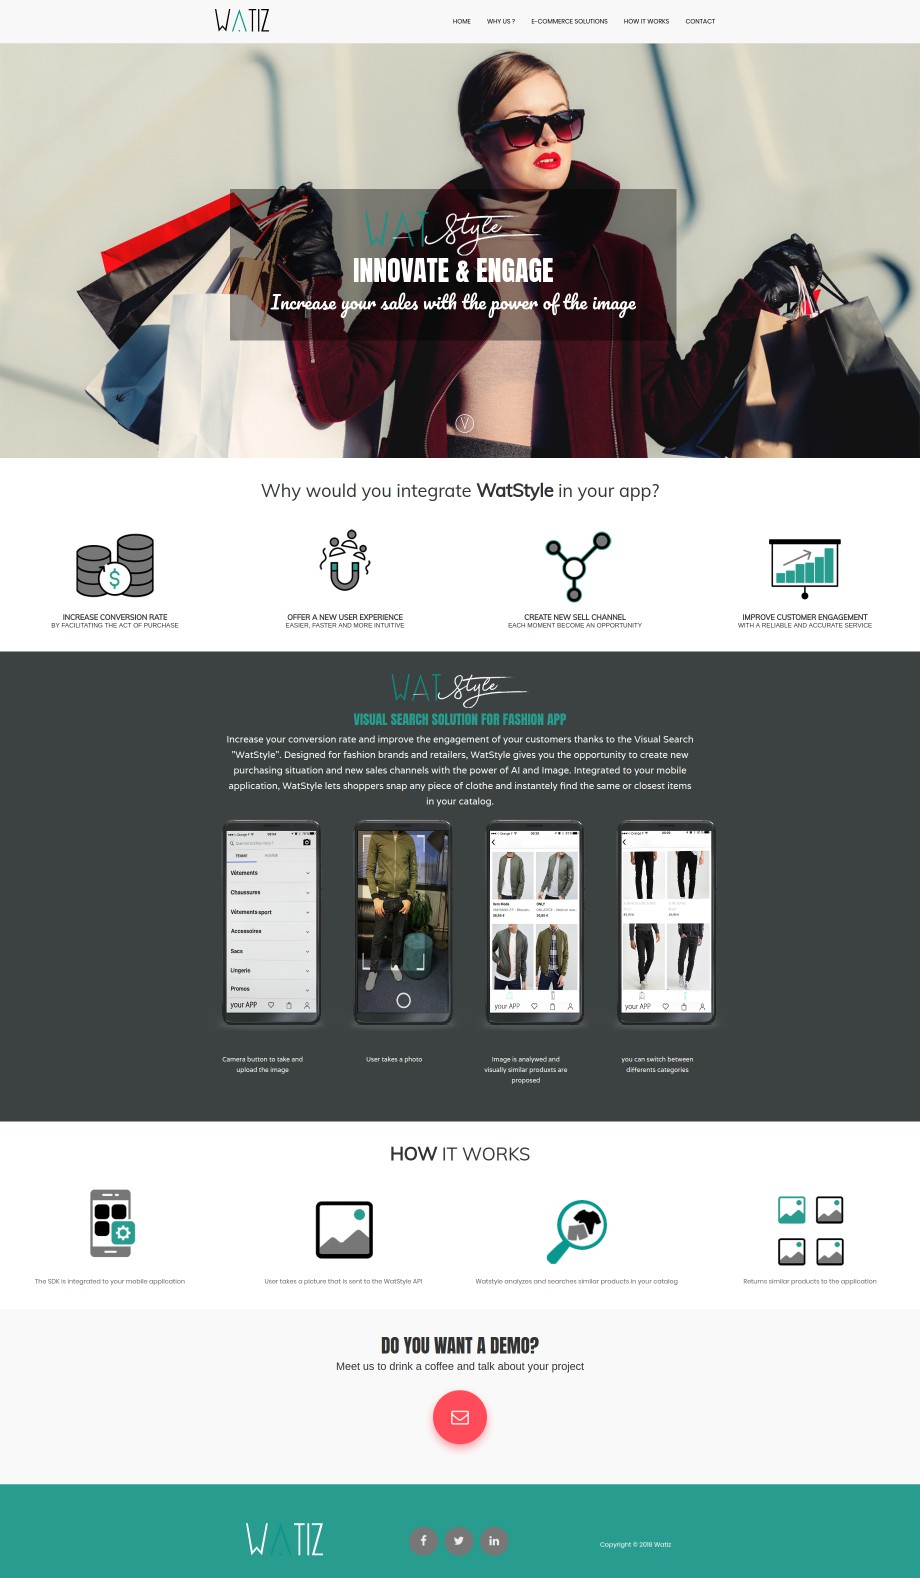
\includegraphics[height=10.2cm]{images/Watstyle.jpg}}
  \caption{Les deux sous-pages}
  \label{fig:4.11}
\end{minipage}
\end{figure}

%%%%%%%%%%%%%%%%%%%%%%%%%%%%%%%%%%%%%%%%%%%%%%%%%%%%%%%%%%%%%%%%%%%%%%%%%%%%%%%%%%%%
\chapter{ Bilan et conclusion}
\section{Bilan professionnel}
Ce stage m’a apporté une nouvelle expérience professionnelle enrichissante. Grâce à ces deux mois passés au sein de la société Watiz, j’ai acquis de nouvelles connaissances autant sur le milieu de l’entreprise que sur les langages informatiques. Le stage dans un milieu professionnel est constructif. En effet, j’ai pu développer mes compétences professionnelles grâce à l’environnement dans lequel j’ai effectué mon stage. J’ai eu la charge de la conception d’un site, du cahier des charges à la réalisation tout en respectant les éléments et les souhaits formulés par les responsables de la société. Tous les objectifs du cahier des charges ont été respectés. J’ai pu développé mes connaissances des langages JS, HTML et CSS ainsi que mes connaissances en gestion. J’ai bien entendu rencontré quelques problèmes lors de la conception du site tels que le mauvais encodage de certains fichiers, les erreurs générées par le JavaScript ou ceux liés au responsive design. Ces problèmes ont tous été résolus et m’ont également apporté de nouveaux savoirs. 
\section{Bilan personnel}
Ce stage a été très enrichissant pour moi car il m’a permis de découvrir dans le détail le développement web front-end. Il m’a permis de participer concrètement aux enjeux de la société Watiz au travers de mes missions variées comme celle du développement de leur site web que j’ai particulièrement apprécié et le projet POC Epick.

Ce stage m’a aussi permis de relever un réel défis pour moi en travaillant sur la généralisation d'un code que je n'ai pas crée initialement. Ceci m'a demandé de lire attentivement le code, comprendre toutes les fonctions et les variables.\\
J'ai aussi appris beaucoup de l'expérience des autres, appris à mieux travailler en équipe en partageant les tâches, les ressources de travail, les connaissances, les opinions et les expériences personnelles.\\
J'ai amélioré mon expression orale en participant aux stand-up's quotidiens où je devais décrire ce que j'ai fait, ce qui me restait à faire et les problèmes rencontrés lors de la réalisation d'une tâche. 
J’ai aussi pu découvrir la vie au sein d’une entreprise. Le fait de se référer à un tuteur constitue une aide dont je n’aurais pu me passer et s’adresser à un supérieur hiérarchique en construisant une explication et une argumentation a été instructif.
\\


 
\section{Conclusion}
En conclusion, la société Watiz dispose maintenant d’un site fonctionnel répondant à toutes leurs attentes et actuellement en ligne. 
Ce stage m’a énormément appris. J'ai ainsi amélioré ma capacité à apprendre rapidement un nouveau langage informatique et j'ai augmenté ma capacité d'analyse face à un problème à résoudre. 
La principale difficulté de ce stage a été pour moi la communication orale à laquelle j'ai consacré beaucoup d'efforts. 
L’entreprise Watiz qui m’a accueilli pendant ce stage fait face à une période charnière sur la promotion de leur produit, et je suis très fier d’avoir pu contribuer et participer à cette révolution.\\

Fort de cette expérience, j’aimerai beaucoup par la suite essayer de m’orienter via un prochain stage, vers le développement web back-end afin d'avoir une vision globale de la création d'un projet web. 

% \nocite{*}
% \bibliographystyle{plain}
% \bibliography{biblio} 
% \phantomsection 
\addcontentsline{toc}{chapter}{Bibliographie} 
\begin{thebibliography}{9}
\bibitem{0}
Bérangère D'Henry. \emph{La recherche visuelle de produits }.
\href{https://blog.sensefuel.com/la-recherche-visuelle-de-produits-les-images-plutot-que-les-mots}{https://blog.sensefuel.com/}, [2018].
\bibitem{1}
Laurène Castor. \emph{UX design : découvrez les fondamentaux }. 
\href{https://openclassrooms.com/courses/decouvrez-les-fondamentaux-de-l-ux-design}{OpenClassRoom}, [2018].
\bibitem{2}
Benoit Gaillat. \emph{Devenir mobile first doit être votre objectif en 2018}. 
\href{http://mobibot.io/blog/420/devenir-mobile-first-doit-etre-votre-objectif-en-2018.html}{http://mobibot.io}, [2017].
\bibitem{3}
Emily Reese. \emph{Découper et intégrer une maquette}.
\href{https://openclassrooms.com/courses/apprenez-a-creer-votre-site-web-avec-html5-et-css3}{https://openclassrooms.com/courses}, [2017].
\bibitem{4}
Mathieu Nebar. \emph{Apprenez à créer votre site web avec HTML5 et CSS3 }.
\href{https://openclassrooms.com/courses/apprenez-a-creer-votre-site-web-avec-html5-et-css3}{OpenClassRoom},[2018].
\bibitem{5} 
Bootstrap. \href{https://getbootstrap.com/docs/4.1/getting-started/introduction/}{Bootstrap Documentation https://getbootstrap.com/}, [2018].
\bibitem{6} 
W3schools. \emph{JavaScript tutoriel}, \href{https://www.w3schools.com/jS/default.asp}{https://www.w3schools.com/jS}, [2018].
\bibitem{7} 
jQuery. \emph{La biblioteque jQuery}\href{https://jquery.com/}{ https://jquery.com/}, [2018].
\bibitem{8}
NPMJS, \emph{html form send email via google script without server}.
\href{https://npmjs.com/package/html-form-send-email-via-google-script-without-server}{https://npmjs.com}, [2018].

\end{thebibliography}
\end{document}
